\chapter{Performance Prediction: Under-, Properly-, or Over-Processed?}
\label{ch:scale-aware}
%\chapter{Scale-aware Hierarchical Image Segmentation} 

\section{Introduction}
\label{sec:intro}
Generic image segmentation has been part of computer vision and image processing communities since the
advent of these fields many decades ago.
The definition of the problem, although vague, is easy to give and understand: ``to divide the pixels of an
image into different pieces, where each piece represents a distinguished \textit{thing}
in the image.''
Martin \etal~\cite{Martin2001} provided these instructions to annotators to create
the Berkeley Segmentation Database (BSDS), which proved that the problem of image segmentation was,
indeed, well defined, as humans provided consistent partitions of the images \textit{up to refinement}.
In other words, image segmentation is inherently a multi-scale problem.

We refer to \textit{flat} image segmentation techniques as those whose output is a single partition of the
image pixels into sets~\cite{shi2000normalized,Comaniciu2002,felzenszwalb2004efficient}.
In these cases, in order to capture the aforementioned multi-scale nature of objects,
one needs to sweep different parameterizations to obtain multiple partitions that contain the
different scales when working with flat segmentation techniques.

On the other hand, hierarchical segmentation produces a single multi-scale structure that aims
at capturing the objects at all scales~\cite{arbelaez2011contour,kim2013learning,Salembier2000,Ren2013,arbelaez2014multiscale}. 
These types of structures have been successfully used in image filtering~\cite{Salembier2000},
semantic segmentation~\cite{Lempitsky2011}, object proposals generation~\cite{arbelaez2014multiscale},
or video segmentation~\cite{xu2013flattening,Varas2015}.

\begin{figure}
\begin{center}
\begin{minipage}{0.24\linewidth}
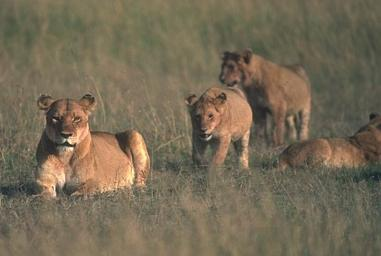
\includegraphics[width=\linewidth]{scale-aware/fig/aligned_lions/cropped_image.jpg}
\end{minipage}
\begin{minipage}{0.24\linewidth}
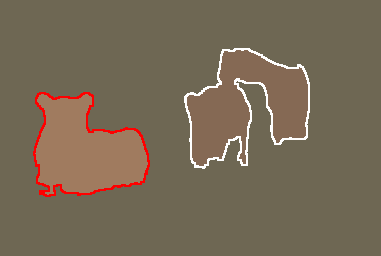
\includegraphics[width=\linewidth]{scale-aware/fig/aligned_lions/mcg_underseg.png}\\[1mm]
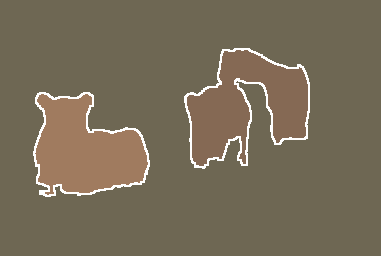
\includegraphics[width=\linewidth]{scale-aware/fig/aligned_lions/mcg_our_underseg.png}
\end{minipage}
\begin{minipage}{0.24\linewidth}
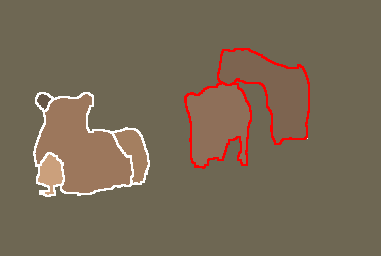
\includegraphics[width=\linewidth]{scale-aware/fig/aligned_lions/mcg_mid.png}\\[1mm]
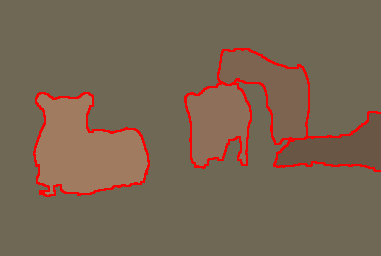
\includegraphics[width=\linewidth]{scale-aware/fig/aligned_lions/mcg_our_good.png}
\end{minipage}
\begin{minipage}{0.24\linewidth}
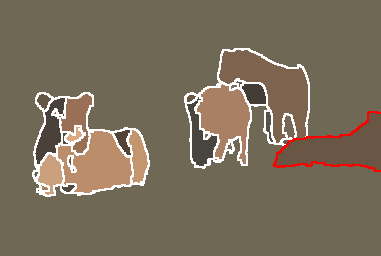
\includegraphics[width=\linewidth]{scale-aware/fig/aligned_lions/mcg_overseg.png}\\[1mm]
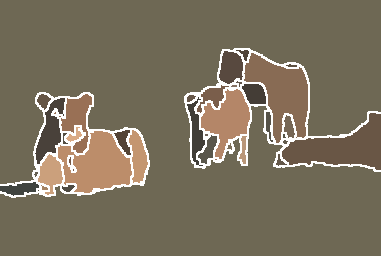
\includegraphics[width=\linewidth]{scale-aware/fig/aligned_lions/mcg_our_overseg.png}
\end{minipage}
\end{center}
\vspace{-2mm}
\caption{\textbf{Example of improved hierarchy alignment}: The original hierarchy (top row) needs three
different flat partitions to represent the four objects (highlighted in red).
Our aligned hierarchy (bottom row) correctly puts all objects in the same level.}
\vspace{-2mm}
\label{fig:thresh_seg}
\end{figure}

The representation power of these hierarchies comes at a cost, however, which is the
difficulty to handle them from a practical (coding) point of view.
While a flat partition can be represented by a matrix of labels of each pixel,
hierarchical structures need a much more complex representation. 
In this context, the Ultrametric Contour Map (UCM)~\cite{arbelaez2011contour} representation is the one that 
gained more traction and it is widely used in the literature.
In it, \textit{flattening} the hierarchy can be achieved by simply \textit{thresholding} the UCM.

The process of \textit{flattening} or \textit{pruning} a hierarchy is therefore of paramount importance for
segmentation, because it is the main proxy used towards the final application.
This work presents a novel technique to improve the flattening of any given hierarchy, that is, 
to get better flat partitions from the same hierarchical segmentation.

\begin{figure*}
\begin{center}
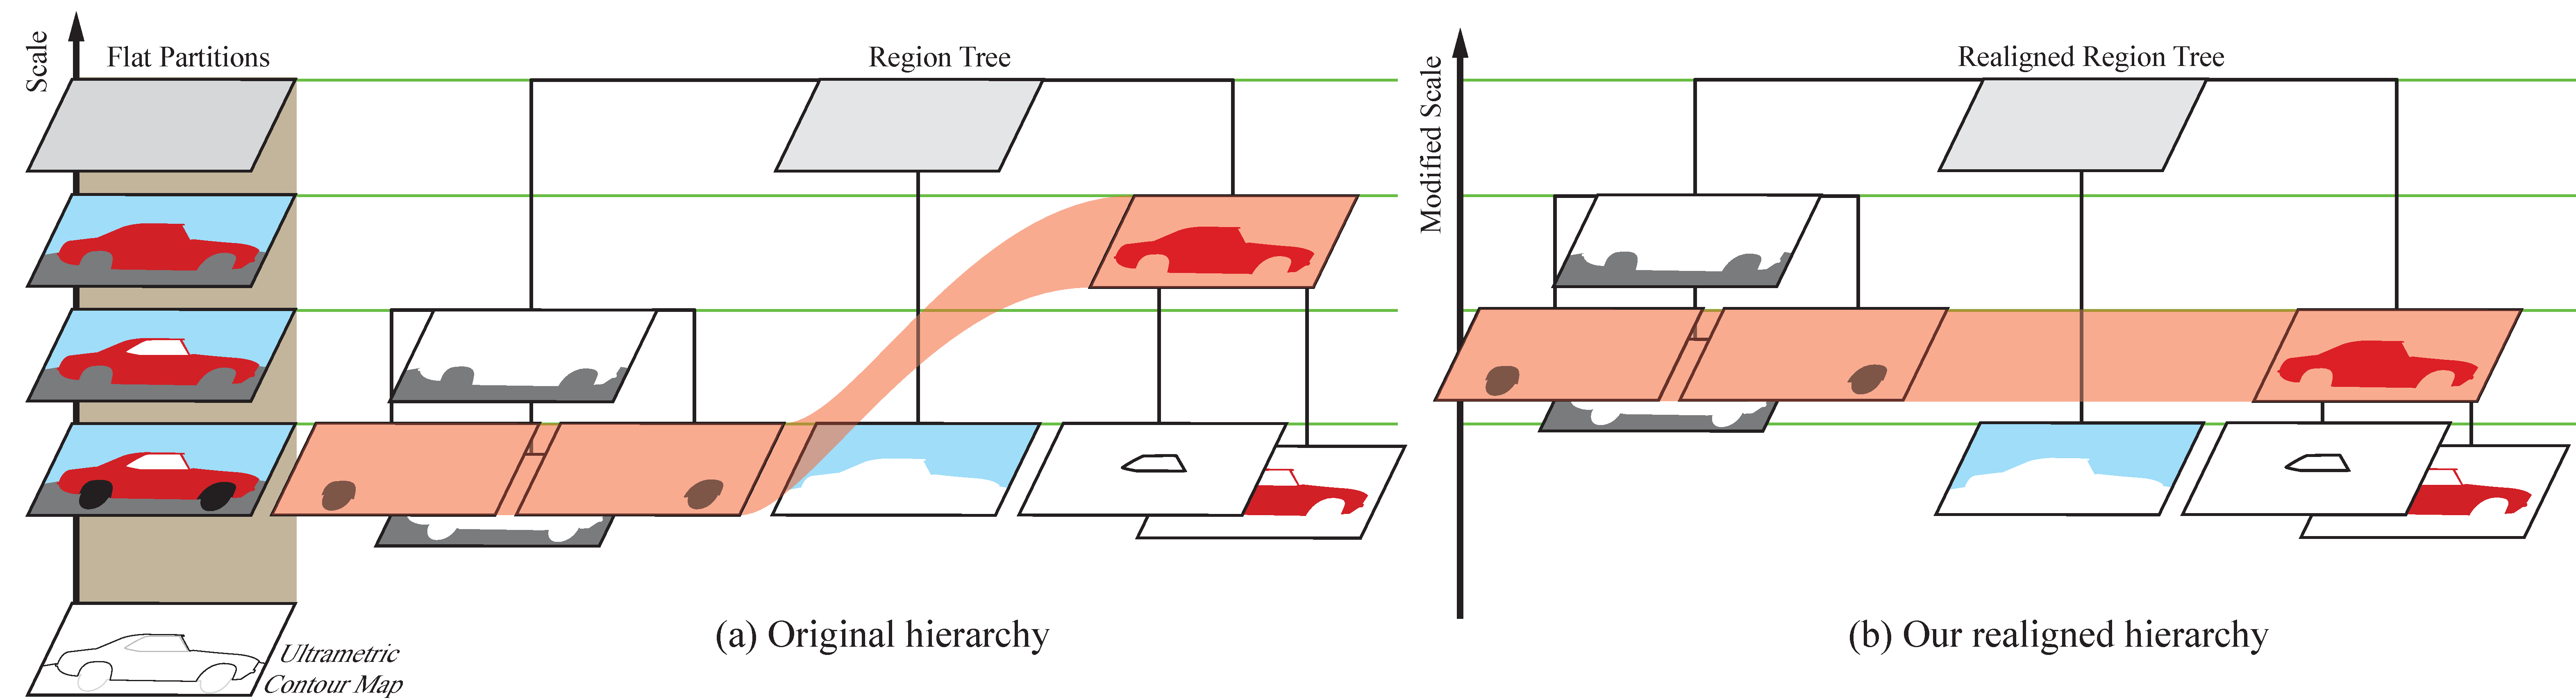
\includegraphics[width=\textwidth]{scale-aware/fig/hierarchy.pdf}
\end{center}
\caption{\textbf{Our proposed hierarchy realignment}: Given a hierarchy (a) in which the objects at the same scale are not well aligned (represented in the same scale level), we produce a realigned hierarchy (b) that
has the similar-scale regions in the same level.}
\label{fig:hier_align}
\end{figure*}

Figure~\ref{fig:thresh_seg} motivates this work.
In the first row we can see different flat partitions extracted from the same hierarchy.
To get the regions representing the four lions we need to search in three different flat partitions, 
extracted at three different levels of the hierarchy.
The second row shows our results, where the same hierarchy is \textit{aligned} to have all objects represented in the same flat partition.

In other words, the threshold level of the hierarchy better relates with the scale of the objects, not only
in the same image, but also across images.
To further grasp the intuition of our work, Figure~\ref{fig:hier_align} shows a UCM and its interpretation as
a region tree (a).
In it, the needed regions to form the car are spread into different scale levels (thresholds of the UCM), as
marked by the red band.
Our proposed realigned hierarchy (b) aims at containing them all in the same scale.

Since the hierarchies are constructed based on low-level features (edges or color), the scale of the objects
is not imposed to be coherent.
We propose to learn the concept of object scale from mid-level features within the hierarchy.
Our objective is to take advantage of these mid-level features as much as possible without getting to
high-level features that would allow us to go beyond scale.
This way, the global approach would be to construct the hierarchies using low-level features,
and then exploit mid-level features to realign them, thus taking the maximum advantage of the most simple 
features possible.

Our alignment also aims at providing a global alignment among different images, that is, providing levels 
of scale that keep meaning even when changing images, allowing higher-level methods to generalize in a more straightforward manner.
Specifically, we train a regressor to predict whether each region of the hierarchy is oversegmented, undersegmented, or correctly segmented; and we rescale the hierarchy according to the prediction 
of this classifier.
Back to the example in Figure~\ref{fig:thresh_seg}, the majority of regions in the first column (bottom) 
are undersegmented, in the middle column they are correctly segmented, and oversegmented in the last column.

We perform comprehensive experiments on BSDS500 using four different hierarchical segmenters.
We obtain consistent improvements on all hierarchies which proves the usefulness of our approach and its 
generalization power.
The remainder of the paper is organized as follows.
First, Section~\ref{sec:related} gives a brief overview of the related work.
Then Section~\ref{sec:scaling} presents our algorithm for re-scaling and aligning hierarchies.
We demonstrate the effectiveness of our method in the experiments in Section~\ref{sec:experiments} and draw 
the conclusions in Section~\ref{sec:conclusions}.
 
%\yh{following is the old introduction}

%Hierarchical segmentation decomposes a given image into a hierarchy of regions, with the constriant that regions in the lower level are the subparts of higher level. Hierarchical segmentation is commonly represented as an ultrametric contour map (UCM), where different levels of segmentation can be produced by applying certain threshold to UCM. Flat segmentation can be extracted by thresholding the UCM at different scales.
%
%For many vision applications, an input of flat segmentation is required\todo{add some refs}. Thus how to choose proper threshold becomes an important issue. Threshold chosen improperly may result in unsatisfactory segmentation. As can be seen from Fig~\ref{fig:thresh_seg}, too fine a scale will break a region into many small pieces, too coarse a scale will mix different regions together. A common practice is to fix an optimal-dataset-scale(ODS) beforehand based on a group of training images. However, in practice it is unlikely that a single setting of parameters will produce best segmentation result for any general images. In order to achieve optimal result, it takes significant amount of human efforts to tune optimal-image-scale(OIS) for each image. Besides, in some case, no single segmentation is capable of capturing all the regions. For example, there are four lions in Fig~\ref{fig:fail_seg}. Each single segmentation can capture one or two lion. But all the segmentations failed no matter how to choose the scale. 
%
%Though its siginificant importance, the problem of how to flatten a hierarchy into a flat segmentation has long been ignored. In this work, instead of choosing one optimal scale, we aim to take leverage of the rich multiscale information stored in the segmentation hierarchy.  The key idea of our work is to save all the good segments in different scale, and combine them into a single segmentation. Specifically, we learn to identify a group of potential scale that may includes useful regions for each specific image. Then we make use of mid-level and high level features to predict the quality of regions. In order to flatten segmentation hierarchies, we develop a simple and efficient algorithm to merge different scales greedily based on the score predicted before.
%
%We conduct extensive experiments on the BSDS500 dataset, and NYC dataset~\todo{add later}.   

% The underlying assumption is that there is a common parameter for all the images. However, the assumption barely holds in practice due to large diversity in natural images. Another 




\section{Related Work}
\label{sec:related}
\paragraph{Hierarchical Segmentation}
There is a rich literature of hierarchical segmentation.
As stated in the introduction, our focus in this paper is not to develop a better hierarchical
segmentation algorithm, but to provide a better alignment of a given hierarchy. 
%Therefore we give a brief review of several most popular approaches.
Hierarchical segmentation typically starts from various local information embedded in an affinity matrix,
such as Pointwise Mutual Information~\cite{isola2014crisp}, or multiscale local brightness, color, and texture cues~\cite{arbelaez2011contour}.
It then greedily constructs a hierarchy of regions by iteratively merging the most similar sets of regions
according to a certain metric. 
The result of hierarchical segmentation is commonly represented as an Ultrametric Contour Map (UCM),
where different levels of segmentation can be produced by applying different thresholds to UCM.
This work proposes to realign the hierarchies in order to make the thresholds of the UCM more closely related
to the scale of objects.
Hierarchical segmentation has become the major trend in image segmentation and most of top-performance segmenters~\cite{arbelaez2011contour,arbelaez2014multiscale,Ren2013,kim2013learning} fall into this category. 
%Particularly we use~\cite{arbelaez2011contour,arbelaez2014multiscale} as our input due to their popularity in many other vision applications. Also options are also possible for our system. 

\paragraph{Multiple Segmentations}
Working with multiple segmentations at the same time has been used in the computer vision community
for a long time, with the idea that, while none of the segmentations is likely to partition the image perfectly, some parts in some segmentations might be useful.
Hoiem \etal~\cite{hoiem2005geometric} use this idea to estimate the scene structure.
A similar idea was exploited by Russell \etal~\cite{russell2006using} to discover objects,
and by Malisiewicz \etal~\cite{malisiewicz2007improving} to improve the spatial support of regions for
recognition.
By realigning the hierarchies we aim to minimize the number of partitions from a hierarchy needed to obtain
reasonable results, since we concentrate same-scale regions in the same partition.
%We have the similar philosophy with previous works. Instead of choosing one optimal scale, we aim to take leverage of the rich multiscale information stored in the segmentation hierarchy. 
Our work also shares some similarities with~\cite{xu2013flattening}, where they flatten supervoxel
hierarchies in videos by finding a slice with uniform entropy.

%However, they formulate the problem as a quadratic integral programming, which makes the optimization NP-hard.
%On the contrary, we use a simple yet effective dynamic programming algorithm to find a globally-optimal slice.  

\paragraph{Predicting Segmentation Quality by Classification}
Classification has been exploited to predict segmentation quality in many works.
Ren \etal~\cite{ren2003learning} use a linear classifier base on Gestalt features~\cite{palmer1999vision}
to distinguish good and bad segmentations.
Their negative training data are generated by randomly placing a ground-truth mask over an image.
A similar idea is used to select parameters by Peng \etal~\cite{peng2008parameter} to select $\lambda$ in 
graph-cut based interactive segmentation.
They compute the segmentation with different $\lambda$, then select the one with highest predicted quality. 
More recently, Carreira \etal~\cite{carreira2010constrained}, Arbelaez \etal~\cite{arbelaez2014multiscale},
and Endres \etal~\cite{endres2014category} use a regression forest to predict the good overlap between
segments (object proposals) and ground truth objects.
We use similar features to~\cite{carreira2010constrained}, which are based on graph partition properties,
region properties, and Gestalt properties.
%Our work also share some similarities with~\cite{peng2008parameter}, where they use a regressor to decide quality of each parameter, and choose the one with highest score.

   
\paragraph{Scale-aware Vision Algorithms} 
Our work also bear a resemblance to the scale-aware algorithms for other vision tasks. 
For instance, exploiting the scale information has proven helpful for semantic image segmentation~\cite{chen2015attention} and 
pedestrain detection~\cite{li2015scale}. \cite{SR4VTs:wacv16} show that 
vision algorithms employing super-resolved images (higher-resolution) perform better than using low-resolution images directly.  
Other scale-aware applications include object tracking~\cite{Klodt2013} and image thumbnailling~\cite{Sun2013}.     
   
   
   
   
   
   %\section{Critical Levels}

There are around 500 different layers, and XXX regions in a single segmentation tree. Besides, regions in nearby layer can be highly similar. Assessing all of them is both unnecessary and computationally impractical. Therefore, as a pre-processing step, we aim to predict a set of critical levels. These critical levels should be complementary to achieve a high recall to ground truth regions, yet keep the size of set smaller. Similar idea was used in~\cite{krahenbuhl2014geodesic}, where they use critical levels to predict size of segmentation masks.

In order to identify these critical levels efficiently, we train a model based on segmentation entropy features. Segmentation entropy of a segmentation $S$ is defined as:
\begin{equation}
Entropy(S) = \sum_{\textbf{r}\in S}{|\textbf{r}|log(|\textbf{r}|)}
\end{equation}

$|\textbf{r}|$ represents the area of a region $\textbf{r}$ in segmentation $S$. Since only the area is required, segmentation entropy is very fast to compute. It enables us to assess difference between layers of a segmentation tree efficiently, as illustrated in Fig~\ref{fig:entropy}. The steep point on the curve indicates there is a large change in the segmentation.

\begin{figure}
\begin{center}
\includegraphics[width=0.5\linewidth]{fig/6046_ucm.png}
\end{center}
\caption{entropy}
\label{fig:entropy}
\end{figure}

The features used includes: value of threshold and entropy, and local gradient of both threshold and entropy calculated with different footstep length. More details about the feature are in the supplementary materials.

\yh{Experiments are not done, will add later}
  
\section{Flattening and Re-scaling  Hierarchies}
\label{sec:scaling}
As discussed in the introduction, while segmentation
hierarchies contain a rich multiscale decomposition of the image, it is
not trivial to distill such knowledge because the hierarchies
generated by current methods are not fully scale-aware. Simply taking
a layer yields a segmentation of which some parts are under-segmented
while others are over-segmented. In this section, we present our
method which aligns the scales of segmentation hierarchies, making
image hierarchies easier to use in practice. We start with scale
labeling, and then present the alignment strategy.


\subsection{Flattening Hierarchies via Scale Labeling}
\label{sec:scale:labeling}


\begin{figure}
\begin{center}
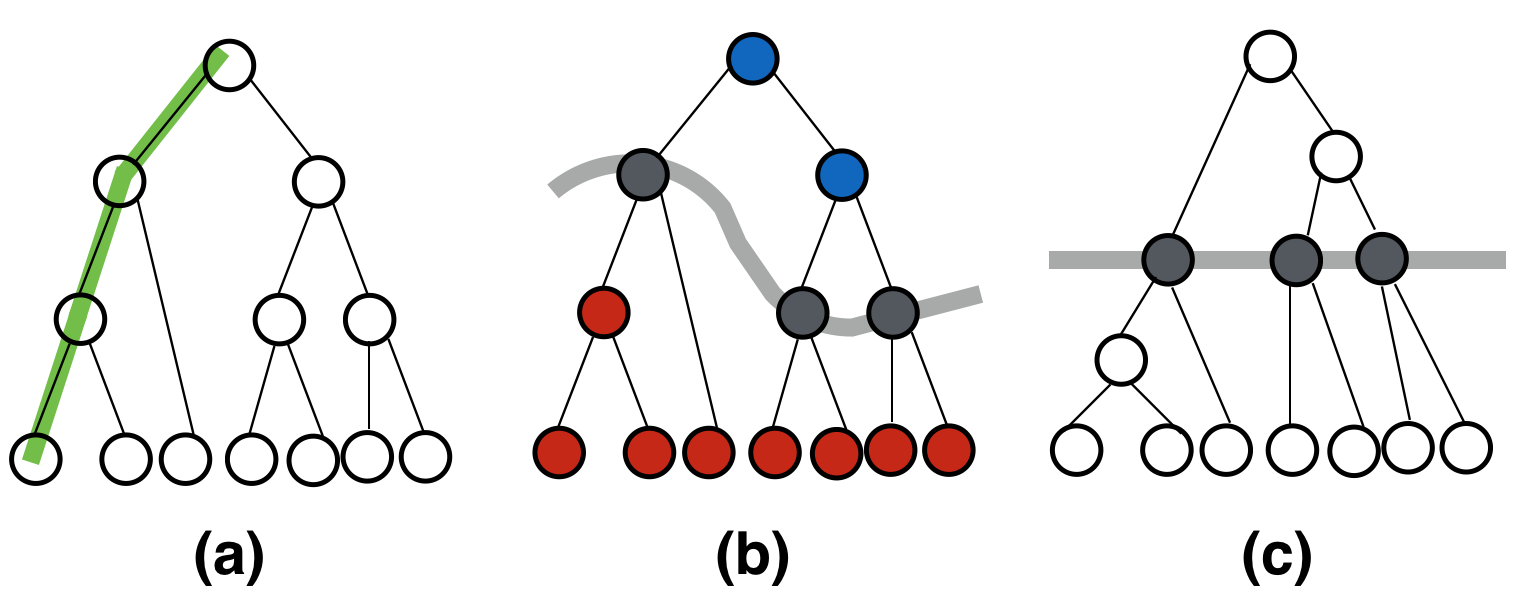
\includegraphics[width=0.7\textwidth]{scale-aware/fig/illu.png}
\end{center}
\caption{Examples of the slices and paths of the segmentation tree,
  where one path of the tree is shown in green (a) and one slice is shown
  in grey (b).  In (b), all nodes
  in blue are in $\mathcal{L}^-$, and all nodes in red are in
  $\mathcal{L}^+$. Our approach re-aligns the hierarchy using the
  anchor slice. The aligned tree is shown in (c).}
\label{fig:hier_opt}
\end{figure}


% We restrict to the the segmentation hierarchy which can be represented
% as a rooted tree, due to its popularity and simplicity. 
Let's denote the segmentation tree of image $I$ by $\mathcal{T}$, with
node $v_i$ indicating its $i$-th node. The nodes correspond to regions
(segments) of $I$.  Given $\mathcal{T}$, our task is to find a tree
slice $\mathcal{L}$ to divide all nodes $v_i$'s (segments) into three
groups: $\mathcal{L}^-$, $\mathcal{L}$, and $\mathcal{L}^+$ indicating
under-, properly- and over-segmented, respectively. See
Figure~\ref{fig:hier_opt}(b) for an example of nodes in the three
groups.

The visual representation of a slice can be seen in Figure~\ref{fig:hier_align}
as red bands covering different regions.
An example of the three types of slices can be found in Figure~\ref{fig:thresh_seg} (bottom row),
where the left partition is mainly oversegmented, the middle one correctly segmented, and the right one undersegmented.

The problem is formulated as a three-class labeling problem.
For each node $v_i$, we use $x(v_i) \in\{-1,0,1\}$ as its class label, with $-1$,
$0$, and $1$ indicating the membership of $v_i$ to $\mathcal{L}^-$, 
$\mathcal{L}$, and $\mathcal{L}^+$ respectively.  Assume now that a
function $f(v_i): v_i \rightarrow [-1, 1] $ is provided to measure the
granularity of image segments, where negative values stand for
under-segmented, $0$ for properly-segmented, and positive for
over-segmented regions.
The magnitude of $f(v_i)$ signals the deviation from being properly-segmented.
Section~\ref{sec:scale} present the proposed learning algorithm for $f(v_i)$.  

The labeling of all $v_i$'s could be done by greedily taking the best-scoring class for each node.
% Thus, the following properties are desired for a good slice: nodes
% above the slice should have $RS$ larger than 0, $RS$ of nodes in the
% slice are close to zero, and below the slice smaller than 0.
However, not any labeling represents a valid slice of the tree.
Following the definition
in~\cite{pont2012supervised,xu2013flattening}, a tree slice is a set
of nodes such that every path $\mathcal{P}_n, n\in \{1,2, ..., N\}$
from the leaf node $\bar{v}_n$ to the root node $v_0$ contains one and
only one node $v$ in the slice. See Figure~\ref{fig:hier_opt} for the
examples of the slices and paths.

From the nature of segmentation hierarchies, the labels of parent nodes $v^p_i$
should be equal or smaller than their child nodes $v_i$.
Intuitively, if a region is correctly segmented, the parent cannot be oversegmented. On the other hand, the parent of an undersegmented region will also be undersegmented.
Putting the two constraints together, the labeling problem can be
formulated as:

% For a valid slice, all nodes in the slice need to be able to form a
% complete segmentation of the tree. We modeled the constraint similar
% to~\cite{pont2012supervised,xu2013flattening}. Given the hierarchy,
% we can specify all the leaf-to-root paths, we donate them as $P =
% \{p_1,\cdots,p_s\}$. For each path, it can be represented as a
% sequence of nodes it has passed through, starts from leaf node and
% ends with the root node $p_i = (v_{i1},v_{i2},\cdots)$. For each
% path in a valid slice, there can be only one node in
% $\mathcal{L}_2$. And a node's label should be smaller or equal than
% the node before it to guarantee the physical meaning of the label.

% \begin{gather}
%  \hat{\mathbf{X}} = \min_{\mathbf{X}} E(\mathbf{X})\\
%  E = \sum_{v_i\in \mathcal{L}_1}{|r_i|\textbf{H}({-s_i}')} + \sum_{v_i\in \mathcal{L}_2}{|r_i|\cdot|{s_i}'|} + \sum_{v_i\in \mathcal{L}_3}{|r_i|\textbf{H}({s_i}')} \\
%  \text{s.t } \forall p_i, \sum_{k}\mathbbm{1}(v_{ik}=2) = 1, \\
%  \forall p_i, x_{i1}\geq x_{i2}\geq x_{i3}\geq \cdots, \\
%  \forall x_i, x_i\in \{1,2,3\}
% \end{gather}


\begin{equation}
  \label{eq:energy}
  \begin{split}
    &\hat{\mathbf{X}} = arg\min_{\mathbf{X}} E(\mathbf{X})\\
 E(\mathbf{X}) =  \sum_{v_i \in \mathcal{L}} &\#(v_i) \cdot \|f(v_i)\|^2 + \lambda  \sum_{v_i \notin \mathcal{L}}  \#(v_i) \cdot l(v_i) \\
 \text{s.t   }  \quad \forall n: & \quad \sum_{v \in \mathcal{P}_n} \mathbbm{1}_\mathcal{L} (v) = 1\\
              \quad \forall v:  & \quad x(v) >= x(v^p)\\
   \end{split}
\end{equation}

where $\#(v)$ is the size (number of pixels) of segment (node) $v$, $\lambda$ is a
weighting value for the two energy terms, and $l(v_i)$ is the loss
function defined for $v_i \in \{ \mathcal{L}^-, \mathcal{L}^+ \}$:
\begin{equation}
  \label{eq:loss:fun}
  l(v_i) = \max(0, f(v_i)\cdot x(v_i)).
\end{equation}
The loss function penalizes two contradictory cases:
(i) segments in the group of under-segmented that receive positive scores; and
(ii) segments in the group of over-segmented that receive negative scores.
The problem will be solved via dynamic programming, as explained in the following section.
% \begin{gather}
%  \hat{\mathbf{X}} = \min_{\mathbf{X}} E(\mathbf{X})\\
%  E(\mathbf{X}) = \sum_{v_i \in \mathcal{L}} S(v_i)\|f(v_i)\|^2 + \lambda  \sum_{v_i \notin \mathcal{L}}  l(f(v_i)) \\
%  \text{s.t  }  \forall n: \sum_{v \in \mathcal{P}_n} \mathbbm{1}_\mathcal{L} (x(v)) = 1\\
%               \forall p_i, x_{i1}\geq x_{i2}\geq x_{i3}\geq \cdots, \\
%  \forall x_i, x_i\in \{1,2,3\}
%  % E = \sum_{v_i\in \mathcal{L}_1}{|r_i|\textbf{H}({-s_i}')} + \sum_{v_i\in \mathcal{L}_2}{|r_i|\cdot|{s_i}'|} + \sum_{v_i\in \mathcal{L}_3}{|r_i|\textbf{H}({s_i}')} \\
%  % \text{s.t } \forall p_i, \sum_{k}\mathbbm{1}(v_{ik}=2) = 1, \\
%  % \forall p_i, x_{i1}\geq x_{i2}\geq x_{i3}\geq \cdots, \\
%  % \forall x_i, x_i\in \{1,2,3\}
% \end{gather}

% In the equation above, $\textbf{H}$ is Heaviside step function and
% $\mathbbm{1}$ is the indicator function. The first two constraints
% ensure the resulted slice is a valid slice. The problem can be viewed
% as a linear integral optimization problem, which is N-P hard in
% general.\yh{really NP-hard?}


\subsubsection{Inference by Dynamic Programming}
\label{sec:dp}
The optimization problem in Equation \ref{eq:energy} is highly structured
and can be solved recursively by Dynamic Programming.
For the subtree rooted at node $v$, its optimal slice $\mathcal{L}(v)$ is either the
node $v$ itself or the union of the optimal slices of all its child
nodes $v^c$'s, depending on whose energy is lower.
Thus, the problem has optimal substructure~\cite{cormen2009introduction}
and so it naturally fits to the framework of dynamic programming to find the global optimal solution. 

% More formally, we can decompose our energy function into two terms:
% \begin{multline}
%  min[E(\mathcal{T}_{root})] = \min\{\sum_{\mathcal{T}_{child}\in\mathcal{C}(\mathcal{T}_{root})}E(\mathcal{T}_{child})+E_1(v_{root}), \\
% 	  E_2(v_{root})+\sum_{v_i \in V\setminus v_{root}} E_3(v_i)\}
% \end{multline}


% There are two
% cases for the root node $v_0$. Either it is in the optimal slice
% $v_{root} \in \mathcal{L}_2$, or it is above the optimal slice
% $v_{root} \in \mathcal{L}_1$. For the first case, except for the root
% node $x_{root}=2$, all other nodes have a label $3$, which indicates
% that they are below the optimal slice. Therefore the energy of the
% tree can be calculated. For the later case, the minimum energy of the
% whole tree is the sum of energy of root node and all minimum energy of
% all its sub-trees.

% The problem can be divided into a set of sub-problems, thus the
% objective can be regarded as a dynamic programming problem. 

% To accommodate our problem of optimizing hierarchy. We propose a greedy
% algorithm similar to~\cite{uijlings2013selective,bonev2014fast}.
The problem proceeds from bottom to the top of the tree.
For each subtree rooted at the current node $v$, the energy of $v \in
\mathcal{L}(v)$ is computed and the energy of the optimal slices of
all its child nodes is requested for comparison.
The algorithm traverses back, and all comparison will be completed when the algorithm reaches the root
node, and the global optimal of Equation \ref{eq:energy} is obtained.
The method is highly efficient with complexity $\mathcal{O}(N)$, where $N$ is the total number of nodes.
The global optimal of the energy can be found by applying Algorithm~\ref{ag:dp} to the root node,
and the optimal slice is the corresponding set of nodes labeled to $0$. 

\begin{algorithm}[tb]
\caption{Dynamic Programming in a Tree}
\label{ag:dp}
\begin{algorithmic}
\STATE \textbf{Input:} tree node $v_i$
\IF{$v_i$ is a leaf node}
\STATE{$\mathcal{C}_{v_i} \gets \#(v_i) \cdot \max(0, f(v_i))$}
\STATE{$E^*_{v_i} \gets \#(v_i) \cdot \|f(v_i)\|^2$}
\ELSE
\STATE $\mathcal{C}_{v_i} \gets  \sum_{v_j \in \{v^c\}}\mathcal{C}_{v_j} + \#(v_i) \cdot \max(0, f(v_i))$
\STATE $E^*_{v_i} \gets min(\sum_{v_j \in \{v^c\}}E^*_{v_j} + \lambda \cdot \#(v_i) \cdot \max(0, -f(v_i)), \#(v_i) \cdot \|f(v_i)\|^2 + \lambda \cdot \sum_{v_j \in \{v^c\}}\mathcal{C}_{v_j})$
\ENDIF
\RETURN $\mathcal{C}_{v_i},E^*_{v_i}$ 
\end{algorithmic}
\end{algorithm}

% 
% \begin{figure}
% \begin{minipage}{.23\textwidth}
% \centering
% 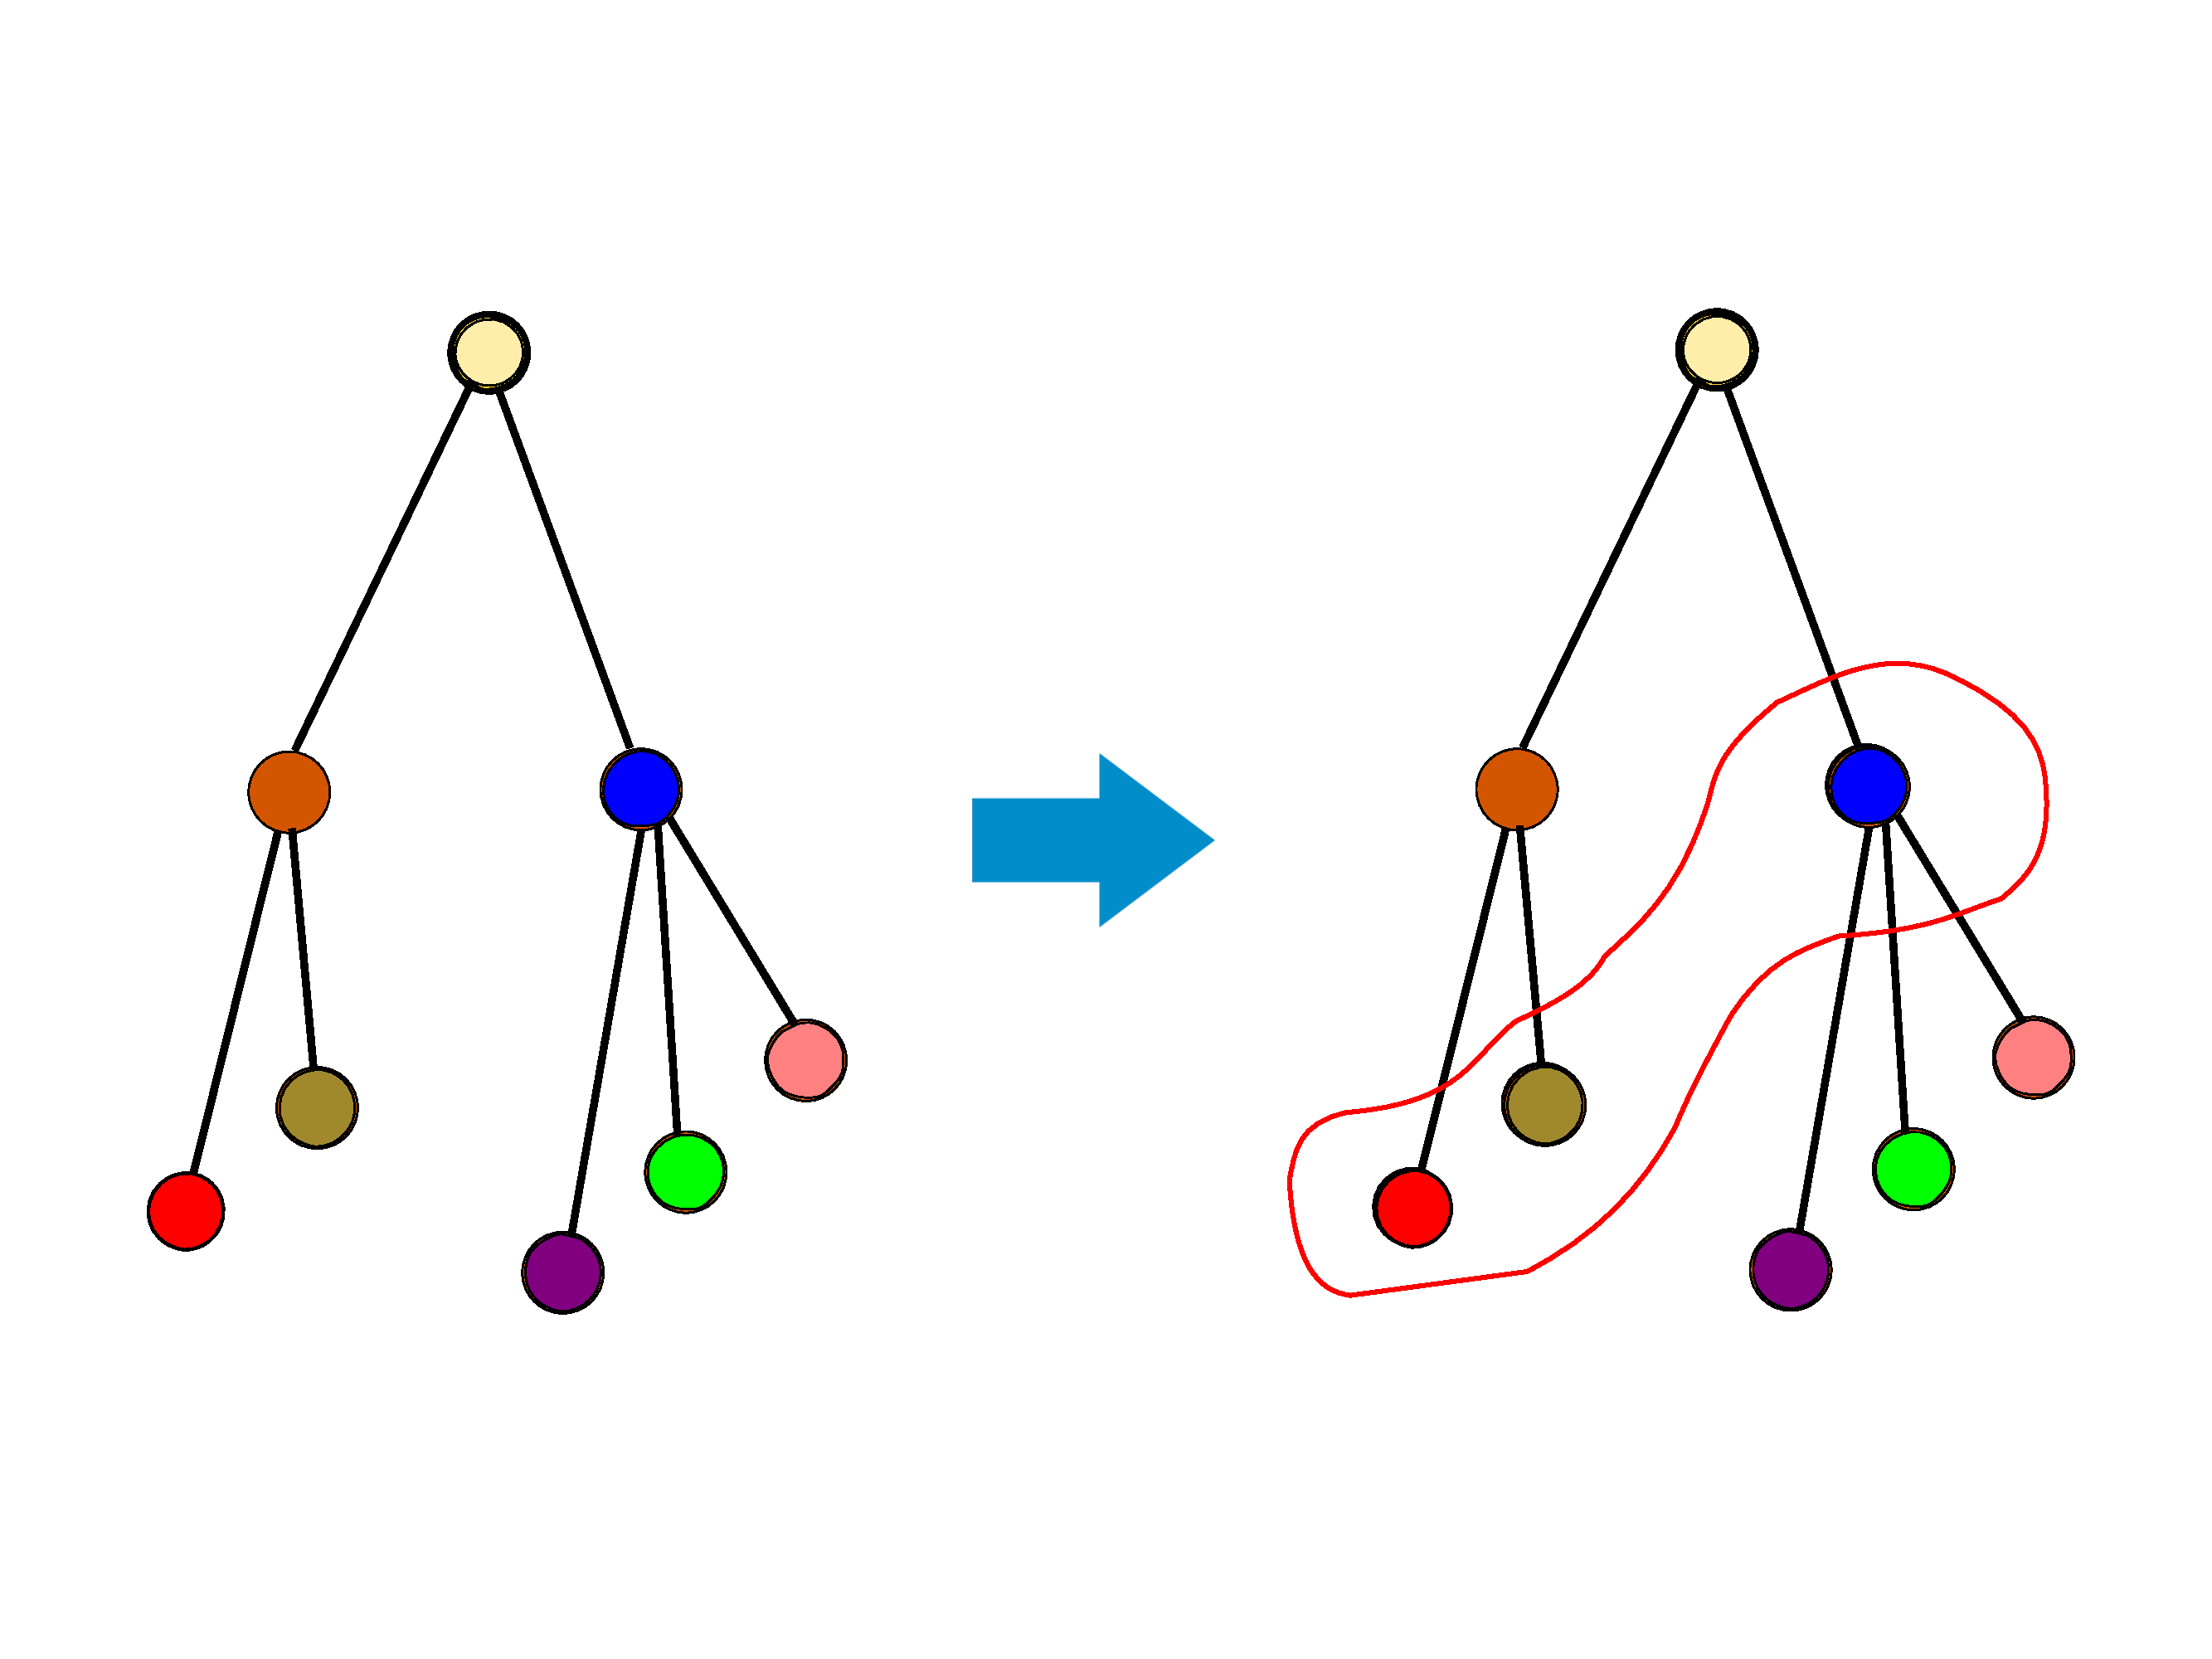
\includegraphics[width=1\linewidth]{scale-aware/fig/syn_hier_1.pdf}
% \end{minipage}
% \begin{minipage}{.23\textwidth}
% \centering
% 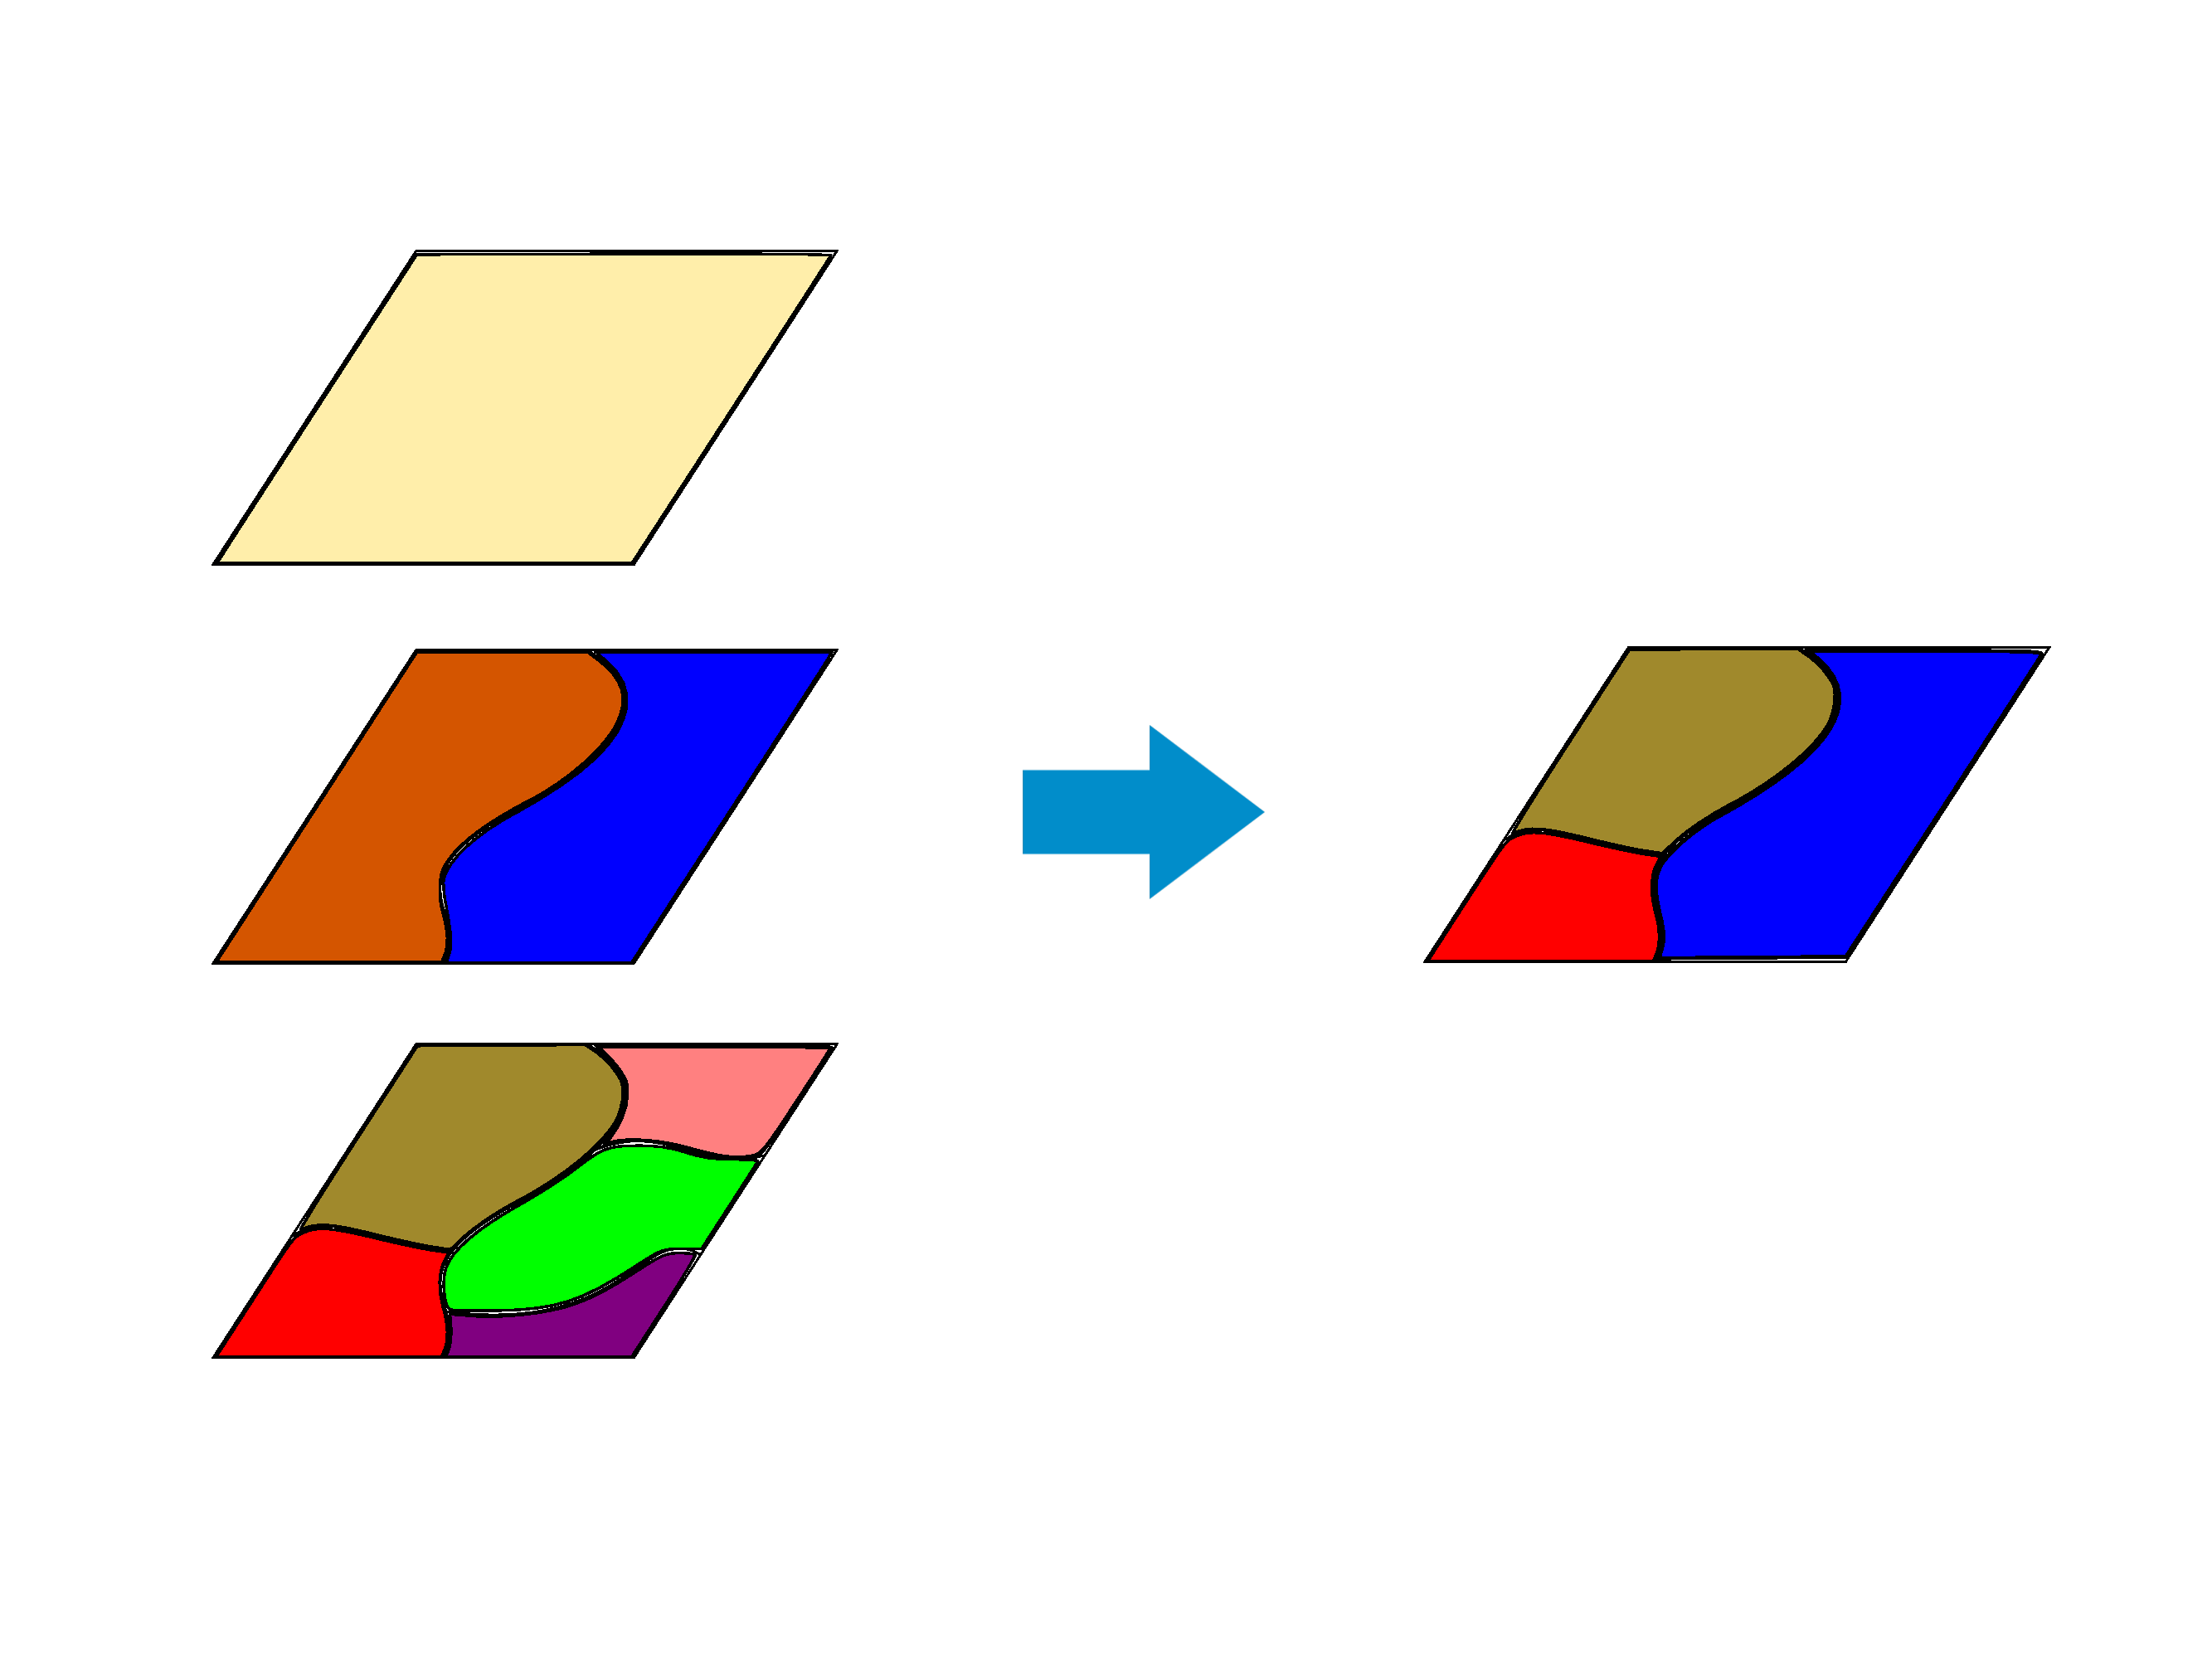
\includegraphics[width=1\linewidth]{scale-aware/fig/syn_hier_2.pdf}
% \end{minipage}
% \caption{The proposed algorithm to flatten hierarchical segmentation.}
% \label{fig:hierseg}
% \end{figure}
% 

\subsubsection{Predicting the Scales of Segments}
\label{sec:scale}
In order to predict the scales (under-, properly-, or
over-segmented) of the segments, we follow the route of modern computer vision
systems to learn a predictor from human-annotated training data.
To this end, we define a measure to compare the scale of an image segment
$\mathbf{r}$ to that of the corresponding human-annotated segment
$\mathbf{g}$.
The correspondence is built up by computing the overlap between computer-generated segments and
human-annotated ones -- the most-overlapping human-annotated segment is taken as the
ground-truth of the computer-generated ones.
The overlap is computed with the Intersection over Union (IoU).
% For each region $\textbf{r}$ in the segmentation tree, we can
% correspond it to the ground truth region $\textbf{g}$ with highest
% overlap, overlap is defined as $O(\textbf{r},\textbf{g}) =
% \frac{|\textbf{r} \cap \textbf{g}|}{|\textbf{r} \cup \textbf{g}|}$. We
% use relative scale($RS$) of a region to its corresponding ground truth
% to indicate the size of region.~\yh{is there any name for this?} 

After having the ground-truth segment $\mathbf{g}$, the scale of the
segment $\mathbf{r}$ is then defined as:
\begin{equation}
\label{eq:scale}
S(\mathbf{r}) = \frac{\#(\mathbf{g}) - \#(\mathbf{r})}{\max( \#(\mathbf{r}), \#(\mathbf{g})))}.
\end{equation}
The value of $S(\mathbf{r})$ is in $[-1, 1]$, with negative values for
\emph{under-}, $0$ for \emph{properly-} and positive values for
\emph{over-segmented} regions, the magnitude of the values representing the extent of being under- or over-segmented, which casts to what we expected from
$f(v)$ (\cf Section~\ref{sec:scale:labeling}). 

With Equation~\ref{eq:scale}, the \emph{scales} of the segments by
segmentation methods can be computed and used as the training data to
train our scale predictor.

As to the learning method, we employ a regression forest as the predictor $f(v)$.
As to the features, we use a set of low-, and middle-level features, mainly following the work
done for object proposals~\cite{carreira2010constrained,arbelaez2014multiscale}.
The features are designed to capture a variety of region properties, and the detailed list of the features is provided in Sec~\ref{sec:settings}.

The main difference between our prediction and the previous
work~\cite{carreira2010constrained, ren2003learning, arbelaez2014multiscale} is that they predict the quality of segments, while we
predict the scale of the segments. Although numerous measures have
been proposed, it is still very hard to quantify the quality of
segments.
The granularity of segments, however, is easier to quantify,
and it also provides more specific information such as under-segmented
or over-segmented.

% The features we used are general features that have been used by many previous works. Our features can be summarized in the following list:

% \begin{description}
%  \item[Graph partition properties]   cut, ratio cut, normalized cut, unbalanced normalized cut. 
%  \item[Region properties]   area, square root of area, ratio of area to image, perimeter, position of the region centroid, bounding box location and size, major and minor axis lengths of the equivalent ellipse, eccentricity, orientation, convex area, Euler number, perimeter and absolute distance to the center of the image.
%  \item[Gestalt properties]    inter-region texton similarity, intra-region texton similarity, inter-region brightness similarity, intra-region brightness similarity, inter-region contour energy, intra-region contour energy, curvilinear continuity, convexity.
% \end{description}

% We adapt the implementation from~\cite{carreira2010constrained} without much tuning and modification. Note the choice of features set is not specific. Other choice of features, including CNN features, is possible and can be integrated in our system seamlessly.
% 
% \subsubsection{Critical Levels for Traning Data}
% 
% There are around 500 different layers, and XXX regions in a single
% segmentation tree. Besides, regions in nearby layer can be highly
% similar. Assessing all of them is both unnecessary and computationally
% impractical. Therefore, as a pre-processing step, we aim to predict a
% set of critical levels. These critical levels should be complementary
% to achieve a high recall to ground truth regions, yet keep the size of
% set smaller. Similar idea was used in~\cite{krahenbuhl2014geodesic},
% where they use critical levels to predict size of segmentation masks.
% 
% In order to identify these critical levels efficiently, we train a
% model based on segmentation entropy features. Segmentation entropy of
% a segmentation $S$ is defined as:
% \begin{equation}
% Entropy(S) = \sum_{\textbf{r}\in S}{|\textbf{r}|log(|\textbf{r}|)}
% \end{equation}
% 
% $|\textbf{r}|$ represents the area of a region $\textbf{r}$ in
% segmentation $S$. Since only the area is required, segmentation
% entropy is very fast to compute. It enables us to assess difference
% between layers of a segmentation tree efficiently, as illustrated in
% Fig~\ref{fig:entropy}. The steep point on the curve indicates there is
% a large change in the segmentation.
% 
% \begin{figure}
% \begin{center}
% \includegraphics[width=0.5\linewidth]{scale-aware/fig/6046_ucm.png}
% \end{center}
% \caption{entropy}
% \label{fig:entropy}
% \end{figure}
% 
% The features used includes: value of threshold and entropy, and local
% gradient of both threshold and entropy calculated with different
% footstep length. More details about the feature are in the
% supplementary materials.
% 
% \yh{Experiments are not done, will add later}
%   

\subsection{Hierarchy Re-scaling with Labeled Scales} 
After setting the optimal slice, we use it as an anchor slice to
stretch the segmentation tree correspondingly. In our experiments, we use the
threshold value of each optimal node as a control point, and linearly
interpolate the original hierarchy.

Segmentation tree can be represented in the form of
Ultra-Contour-Map(UCM)~\cite{arbelaez2011contour}. UCM is a matrix
with the size $(2h-1)*(2w-1)$, where the $h$ is the height of the
original image, and $w$ is the width. Therefore for each pair of
neighboring pixels in the image, the value in the UCM matrix
represents their boundary strength. And usually it is a value between
$0$ and $1$. Segmentation of a certain scale can be extracted by
thresholding the UCM with corresponding value. Without losing any
generality, our algorithm directly manipulate on UCM due to its
popularity and simplicity. The algorithm is summarized in
Algorithm~\ref{ag:rescle}. We assume the functions \textbf{Boundary}
to find the corresponding elements of boundary of a region \textbf{r}
in the UCM matrix, and \textbf{InnerArea} to find its inner area.

\begin{algorithm} [tb]
\caption{Rescaling Hierarchy}
\label{ag:rescle}
\begin{algorithmic}
\STATE \textbf{Input:} Optimal Slice $\mathcal{S}$, UCM map $M_{ucm}$
\FOR{$\textbf{r} \in \mathcal{S}$ } 
\STATE $\textbf{b} \gets \textbf{Boundary}(\textbf{r})$
\STATE $\textbf{a} \gets \textbf{InnerArea}(\textbf{r})$
\STATE $m \gets min(M_{ucm}(\textbf{b}))$
\STATE $M_{ucm}(\textbf{a}) \gets M_{ucm}(\textbf{a})*0.5/m$
\ENDFOR
\STATE $ \textbf{b}_{\textbf{all}} \gets \textbf{Boundary}(\mathcal{S})$
\STATE $m_{min} \gets min(M_{ucm}(\textbf{b}_{\textbf{all}}))$
% \STATE $t_{max} := max(M_{ucm}(\textbf{b}_\textbf{all}))$
\STATE $M_{ucm}(\textbf{b}_{\textbf{all}}) \gets m_{min} + \frac{(M_{ucm}(\textbf{b}_{\textbf{all}})-m_{min})}{2(1-m_{min})}$
\end{algorithmic}
\end{algorithm}

By the presented algorithm, we perform locally linear transform on UCM map, and align the optimal slice to threshold $0.5$, which makes it easier for later use. No information in the original hierarchy is lost during the rescaling process. 




\section{Experiments}
\label{sec:experiments}
We evaluate our approach on the segmentation hierarchies generated by
multiple different segmentation methods, and further examine its
usefulness on the task of object segmentation. The goal is to
demonstrate that the proposed method is able to improve general
segmentation hierarchies and the improvement is reflected to
high-level vision tasks as well.

% In this section, we present our experiments. First we describe the
% settings of our experiments. Next we incorporate our hierarchy
% alignment with MCG~\cite{arbelaez2014multiscale}, which is
% state-of-the-art hierarchical segmentation method. We report our
% results on the BSDS500 dataset~\cite{arbelaez2011contour}, and compare
% the results against other segmentation methods. Then more results of
% incorporating other hierarchical segmentation method are reported to
% validate the generality of our approach. Finally, to demonstrate the
% usefulness of our approach, we also evaluate our approach towards
% object segmentation.

\subsection{Experiment Settings}
\label{sec:settings}
\textbf{Dataset}:
We benchmark the performance of our approach on BSDS500
dataset~\cite{arbelaez2011contour}, which includes 500 images, with
200 for training, 100 for validation, and 200 for testing.  Each image is
annotated by 5 different people on average. As to evaluation, we
deploy three standard metrics: Segmentation Covering (SC),
Probabilistic Rand Index (PRI), and Variation of Information
(VI). Readers are referred to~\cite{arbelaez2011contour} for details
about the dataset and the evaluation metrics.

\textbf{Candidate methods}:
As to the candidate hierarchical segmentation methods, we chose the
following four methods due to their popularity and good
performance:
\begin{itemize}
\item gPb-owt-ucm~\cite{arbelaez2011contour}: a widely-used
  hierarchical segmentation method. Discriminative features are learned
  for local boundary detection and spectral clustering is applied on
  top of it for boundary globalization.

\item MCG~\cite{arbelaez2014multiscale}: a unified framework for
  segmentation and object proposals. It combines information from
  multiple resolutions of the image and achieves the
  state-of-the-art results for both image segmentation and object proposals.

\item SCG~\cite{arbelaez2014multiscale}: the single-resulution,
  faster version version of MCG. It gets competitive results at a fraction of
  the cost of MCG.

\item PMI~\cite{isola2014crisp}: a recent work for unsupervised
  boundary detection. It can be applied for image segmentation as
  well in order to generate a hierarchical segmentation.
\end{itemize}


\textbf{Training}: The training set and the validation set of BSDS500
are pooled together as the training set for our regression forest. The
four segmentation methods are used to generate hierarchies,
over which the training samples (segments) are extracted.
We train method-specific regression forests
as the scale predictor.
Since a large portion of regions in the hierarchies are very small and
features extracted from them are not reliable, we exclude regions smaller
than 50 pixels for the training of the predictor.

Specifically, for each region $\mathbf{r}$, we find its corresponding
ground-truth region $\mathbf{g}$ by taking the human-annotated one with the
highest covering score. 
The relative scale of $\mathbf{r}$ is then computed with
Equation~\ref{eq:scale} for the regression target of $\mathbf{r}$.
As to the features for $\mathbf{r}$, we draw on the
success of object proposals~\cite{carreira2010constrained,arbelaez2014multiscale}.
There, a large pool of middle-level features have been defined for segment description.
The features used are summarized as follows:
\begin{itemize}
\item Graph partition properties: cut, ratio cut, normalized cut, unbalanced normalized cut. 
\item Region properties:  area, perimeter, bounding box size, major and minor axis lengths of the equivalent ellipse, eccentricity, orientation, convex area, Euler number.
\item Gestalt properties: inter- and intra-region texton similarity, inter- and intra-region brightness similarity, inter- and intra-region contour energy, curvilinear continuity, convexity.
\end{itemize}
Readers are referred to~\cite{carreira2010constrained} for the details
of these features. This list is definitely not exhaustive.
More high-level features, \eg by object detection, could be added.

Although these features are simple, extracting them for all layers of
the segmentation hierarchies can be costly.
Doing so is also unnecessary, as most segments at one layer are very
similar to those from the parent layer and the child layer.
Thus, we only extract the features from a subset of layers
sub-sampled from the hierarchies.
The layers are uniformly sampled over the range of UCM values. 

As to the parameters of our method, we set $100$ trees for the random
forest. $\lambda$ in Equation~\ref{eq:energy} is set to $0.1$ to
balance information from the three groups, because there are more
segments over and under the optimal slice $\mathcal{L}$. % than in the slice.
%In our experiments, $\lambda$ is set to $0.1$ to balance our cost. We use 100 trees with default settings in regression forest.

% \begin{description}
%  \item[Graph partition properties]   cut, ratio cut, normalized cut, unbalanced normalized cut. 
%  \item[Region properties]   area, square root of area, ratio of area to image, perimeter, position of the region centroid, bounding box location and size, major and minor axis lengths of the equivalent ellipse, eccentricity, orientation, convex area, Euler number, perimeter and absolute distance to the center of the image.
%  \item[Gestalt properties]    inter-region texton similarity, intra-region texton similarity, inter-region brightness similarity, intra-region brightness similarity, inter-region contour energy, intra-region contour energy, curvilinear continuity, convexity.
% \end{description}

\subsection{Results}
% Our methods can be easily incorporated into any types of hierarchical
% segmentation method. Therefore, these methods can potentially take
% advantage of our approach and benefit from alignment. In order to test
% how well our method generalize to other hierarchical segmenters, we
% conduct the following two experiments: Firstly we evaluate our methods
% on other hierarchies, using the same random forest trained by MCG
% segments. To test whether if a regression forest specifically trained
% can improve the results, in the second experiment, we re-train the
% random forests using segments from each specific algorithms. The
% results are summarized in Table~\ref{tab:res_other_hier}.
The results of our method evaluated on top of the four candidates
segmentation approaches are summarized in
Table~\ref{tab:res_other_hier}. As shown in the table, the
improvements achieved by our alignment are considerable and, more
importantly, they are consistent across different methods.  The method
improves more on ODS than OIS, this is because OIS accesses the
ground-truth segmentations to search for the best-performing
threshold, which somehow diminish the learned knowledge.
We argue that ODS is more practical than OIS in a real vision systems,
because for real applications there is no human-annotated segmentations.

Figure~\ref{fig:visualresult} shows qualitative results of different hierarchies. Our approach shows a consistent improvement over the original results. Since our approach if scale-aware, regions are of similar scale across images after alignment. Thus our method demonstrates better ability of preserving regions across images. In Figure~\ref{fig:mcg_vis2} we show segmentation examples of MCG and
aligned MCG by our method. As the figure shows, the aligned
hierarchies generate characteristics closer to what human expect when
flat segmentations are sampled out of the hierarchies. More
particularly, after alignment, sampled segmentations of the
hierarchies generate consistent responses across all parts of the
image: all parts under-segmented, to all parts properly-segmented, and
finally to all over-segmented while sampling from the top to the
bottom of the hierarchies. This alignment greatly simplifies the use
of hierarchical image segmentation for other vision tasks.
Figure~\ref{fig:visualresult} shows qualitative results with
different hierarchies. Our approach shows a consistent improvement
over the original results. Since our approach is scale-aware, regions
at the same level of the hierarchy are of similar scales across all
areas of the images after the alignment. Thus our method demonstrates
better ability of preserving regions across images.

We also tested the method in the scenario where the random forests are
trained with segments from all of the four methods, and applied to all
of them at test time. This gives slightly poorer results but in turn shows 
that our method can be applied in a method-agnostic approach.
%This can be ascribed to
%the fact that segments from specific methods may own their own
%statistics. Simply mixing them makes the learning tasks more
%challenging.

% This again demonstrate the usefulness of scale
% alignment. Secondly, results can be further improved by training a
% specific random forest. We believe the reason behind this improvement
% is that segments generated by the same region tend to be
% similar.(e.g. Normalized cut tends to break large region, felt-hutt
% segmentation tends to adhere to the boundries) Thus we can take this
% tendency to make more precise prediction if using specific training
% data.
% Qualitative results is shown in Fig~\ref{fig:visualresult}. Our
% method demonstrate better ability to segment regions in different
% scale.

\begin{table}
\begin{center} \small
\resizebox{0.65\textwidth}{!}{
\begin{tabular} {| c | c | c | c | c | c | c |}
\hline
& \multicolumn{2}{c|}{Covering ($\uparrow$)} & \multicolumn{2}{c|}{PRI ($\uparrow$)} 
& \multicolumn{2}{c|}{VI ($\downarrow$)} \\ \cline{2-7}
 & ODS & OIS & ODS & OIS & ODS & OIS \\ \hline
MCG &
0.61  & 0.67  & 0.83  & 0.86  & 1.57  & 1.39  \\
MCG-aligned &
0.63  & 0.68  & 0.83  & 0.86  & 1.53  & 1.38  \\ 
\hline
SCG &
0.60  & 0.66  & 0.83  & 0.86  & 1.63  & 1.42  \\ 
SCG-aligned&
0.61  & 0.67  & 0.83  & 0.86  & 1.61  & 1.41  \\ 
% SCG+ours(retrained)&
% 0.612  & 0.671  & 0.833  & 0.861  & 1.586  & 1.410  \\ 
\hline
gpb &
0.59  & 0.65  & 0.83  & 0.86  & 1.69  & 1.48  \\ 
gpb-aligned &
0.60  & 0.66  & 0.83  & 0.86  & 1.66  & 1.46  \\ 
% gpbours(retrained)&
% 0.608  & 0.663  & 0.828  & 0.858  & 1.642  & 1.460  \\ 
\hline
PMI &
0.53  & 0.59  & 0.76  & 0.81  & 2.03  & 1.80 \\ 
PMI-aligned &
0.54  & 0.59  & 0.76  & 0.81  & 2.01  & 1.80 \\ 
% PMI+ours(retrained)&
% 0.543  & 0.590  & 0.760  & 0.815  & 1.996  & 1.813 \\ 
\hline
\end{tabular}}
\end{center}
\caption{The results of our aligned hierarchies with a comparison to the original hierarchies.}
\label{tab:res_other_hier}
\end{table}

\subsection{Comparison to Other Methods}
As the previous section shows, the MCG aligned by our method generally
performs the best. Here, we compare MCG-aligned to other competing
methods. The results are summarized in Table~\ref{tab:res_bsds} and
demonstrate that segmentation quality can be improved by our
alignment. In particular, the aligned MCG achieves the best result in
Covering and VI. After alignment, the results are on
par with the newest method of PFE+MCG~\cite{yupiecewise}. It is
noteworthy that our method and theirs are complementary, and the
combination of the two may yield even better results. Their method is
to improve feature embedding for a better local distance measure,
while we aim to improve the hierarchy of existing segmentation methods. 

\begin{table}
\begin{center}
\resizebox{0.9\textwidth}{!}{
\begin{tabular} {| c | c | c | c | c | c | c |}
\hline
& \multicolumn{2}{c|}{Covering ($\uparrow$)} & \multicolumn{2}{c|}{PRI ($\uparrow$)} 
& \multicolumn{2}{c|}{VI ($\downarrow$)} \\ \cline{2-7}
 & ODS & OIS & ODS & OIS & ODS & OIS \\ \hline
Ncut~\cite{shi2000normalized} &
0.45  & 0.53  & 0.78  & 0.80 &  2.23 &  1.89 \\
Felz-Hutt~\cite{felzenszwalb2004efficient} &
0.52  & 0.57  & 0.80  & 0.82 &  2.21 &  1.87 \\
Mean Shift~\cite{comaniciu2002mean} &
0.54  & 0.58  & 0.79  & 0.81 &  1.85 &  1.64 \\
Hoiem~\cite{hoiem2011recovering} &
0.56  & 0.60   & 0.80  & 0.77 &  1.78 &  1.66 \\
gPb-owt-ucm~\cite{arbelaez2011contour} &
0.59  & 0.65  & 0.83  & 0.86 &  1.69 &  1.48 \\
ISCRA~\cite{ren2013image} &
0.59  & 0.66  & 0.82  & 0.85 &  1.60 &  1.42 \\
PFE+mPb~\cite{yupiecewise} &
0.62  & 0.67  & 0.84  & 0.86 &  1.61 &  1.43 \\
PFE+MCG~\cite{yupiecewise} &
0.62  & 0.68  & 0.84  & 0.87 &  1.56 &  1.36 \\ \hline
MCG~\cite{arbelaez2014multiscale} &
0.61  & 0.67  & 0.83  & 0.86 &  1.57 &  1.39 \\
MCG+Ours &
0.63  & 0.68  & 0.83  & 0.86 &  1.53 &  1.38 \\
% \textbf{0.62}  & \textbf{0.68}  & \textbf{0.84}  & \textbf{0.87} &  \textbf{1.54} &  \textbf{1.37} \\
\hline
\end{tabular}}
\end{center}
\caption{Segmentation results on BSDS500 test set, with a comparison to the state-of-the-art competitors.}
\label{tab:res_bsds}
\end{table}



\begin{figure*}
\centering
\begin{minipage}{0.48\linewidth}
\resizebox{\linewidth}{!}{%
\begin{tikzpicture}[/pgfplots/width=1.5\linewidth, /pgfplots/height=1.2\linewidth]
    \begin{axis}[ymin=0.2,ymax=0.7,xmin=1,xmax=10,enlargelimits=false,
        xlabel=Number of selected regions,
        ylabel=Jaccard index $J$,
        font=\scriptsize, grid=both,
        legend pos= south east,
        grid style=dotted,
        axis equal image=false,
        title=BSDS500,
        title style={yshift=-1.3ex,},
        ytick={0.1,0.2,...,0.7},
        xtick={1,2,...,10},
        minor ytick={0.1,0.125,...,0.7},
        major grid style={white!20!black},
        minor grid style={white!70!black},
        xlabel shift={-2pt},
        ylabel shift={-3pt}]
         \addplot+[black,solid,mark=none, thick] table[x=mR,y=mJ] {scale-aware/data/BSDS500_val_A-MCG_qual_vs_nregs.txt};
         \addlegendentry{MCG+Our}
         \addplot+[black,dashed,mark=none, thick] table[x=mR,y=mJ] {scale-aware/data/BSDS500_val_MCG_qual_vs_nregs.txt};
         \addlegendentry{MCG}
         \addplot+[blue,solid,mark=none, thick] table[x=mR,y=mJ] {scale-aware/data/BSDS500_val_A-SCG_qual_vs_nregs.txt};
         \addlegendentry{SCG+Our}
         \addplot+[blue,dashed,mark=none, thick] table[x=mR,y=mJ] {scale-aware/data/BSDS500_val_SCG_qual_vs_nregs.txt};
         \addlegendentry{SCG}
         \addplot+[red,solid,mark=none, thick] table[x=mR,y=mJ] {scale-aware/data/BSDS500_val_A-gPb-UCM_qual_vs_nregs.txt};
         \addlegendentry{gPb-UCM+Our}
         \addplot+[red,dashed,mark=none, thick] table[x=mR,y=mJ] {scale-aware/data/BSDS500_val_gPb-UCM_qual_vs_nregs.txt};
         \addlegendentry{gPb-UCM}
         \addplot+[olive,solid,mark=none, thick] table[x=mR,y=mJ] {scale-aware/data/BSDS500_val_A-PMI_qual_vs_nregs.txt};
         \addlegendentry{PMI+Our}
         \addplot+[olive,dashed,mark=none, thick] table[x=mR,y=mJ] {scale-aware/data/BSDS500_val_PMI2_qual_vs_nregs.txt};
         \addlegendentry{PMI}
	 \end{axis}
   \end{tikzpicture}}
   \end{minipage}
   \begin{minipage}{0.48\linewidth}
\resizebox{\linewidth}{!}{%
\begin{tikzpicture}[/pgfplots/width=1.5\linewidth, /pgfplots/height=1.2\linewidth]
    \begin{axis}[ymin=0.2,ymax=0.7,xmin=1,xmax=10,enlargelimits=false,
        xlabel=Number of selected regions,
        ylabel=Jaccard index $J$,
        font=\scriptsize, grid=both,
        legend pos= south east,
        grid style=dotted,
        title=Pascal Segmentation,
        title style={yshift=-1.3ex,},
        axis equal image=false,
        ytick={0.1,0.2,...,0.7},
        xtick={1,2,...,10},
        minor ytick={0.1,0.125,...,0.7},
        major grid style={white!20!black},
        minor grid style={white!70!black},
        xlabel shift={-2pt},
        ylabel shift={-3pt}]
         \addplot+[black,solid,mark=none, thick] table[x=mR,y=mJ] {scale-aware/data/Pascal_Segmentation_val_2012_A-MCG3_qual_vs_nregs.txt};
         \addlegendentry{MCG+Our}
         \addplot+[black,dashed,mark=none, thick] table[x=mR,y=mJ] {scale-aware/data/Pascal_Segmentation_val_2012_MCG_qual_vs_nregs.txt};
         \addlegendentry{MCG}
%         \addplot+[red,solid,mark=none, thick] table[x=mR,y=mJ] {scale-aware/data/BSDS500_val_A-gPb-UCM_qual_vs_nregs.txt};
%         \addlegendentry{gPb-UCM+Our}
%         \addplot+[red,dashed,mark=none, thick] table[x=mR,y=mJ] {scale-aware/data/BSDS500_val_gPb-UCM_qual_vs_nregs.txt};
	 \end{axis}
   \end{tikzpicture}}
   \end{minipage}
       \caption{\textbf{Flattened hierarchies for object detection}: Achievable quality by an oracle with respect to the number of regions needed}
   \label{fig:qual_vs_regs}
\end{figure*}


\begin{figure*}[tb]
\begin{center}
\begin{tabular}{cccccccccc}
\small{Image} &  \small{gpb} &  \small{gpb-R} &  \small{SCG} &  \small{SCG-R} & \small{MCG} & \small{MCG-R} \\   

 \hspace{-2mm}
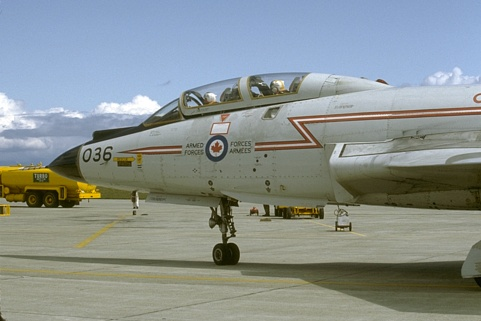
\includegraphics[width=2cm]{scale-aware/fig/visual_result/visual_result_1_1.png}     \hspace{-4mm}
&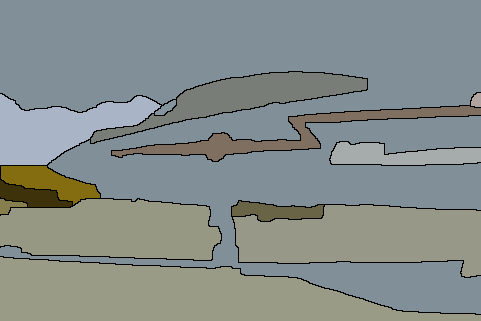
\includegraphics[width=2cm]{scale-aware/fig/visual_result/visual_result_1_2.png} \hspace{-4mm}
&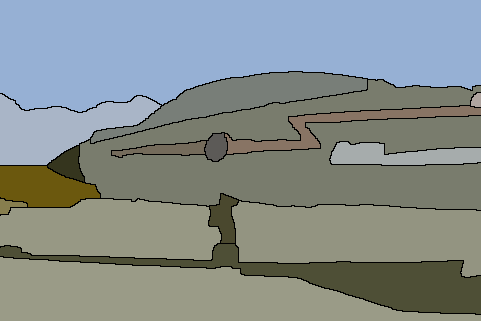
\includegraphics[width=2cm]{scale-aware/fig/visual_result/visual_result_1_3.png} \hspace{-4mm}
&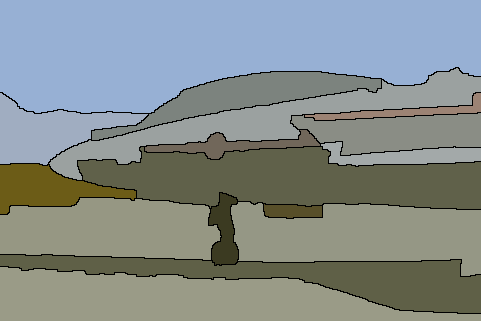
\includegraphics[width=2cm]{scale-aware/fig/visual_result/visual_result_1_4.png} \hspace{-4mm}
&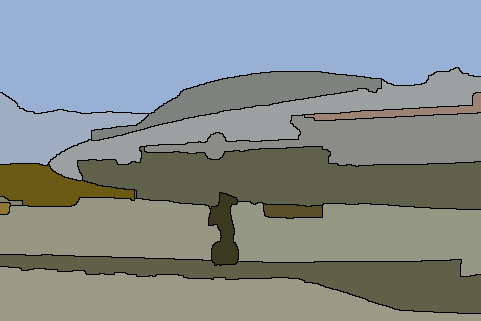
\includegraphics[width=2cm]{scale-aware/fig/visual_result/visual_result_1_5.png} \hspace{-4mm}
&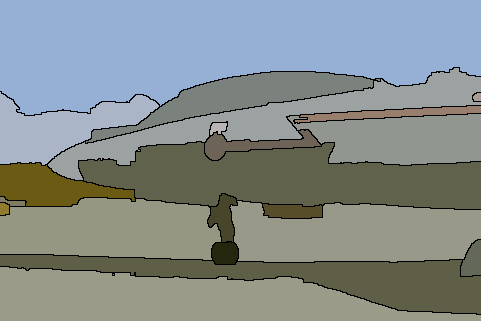
\includegraphics[width=2cm]{scale-aware/fig/visual_result/visual_result_1_6.png} \hspace{-4mm}
&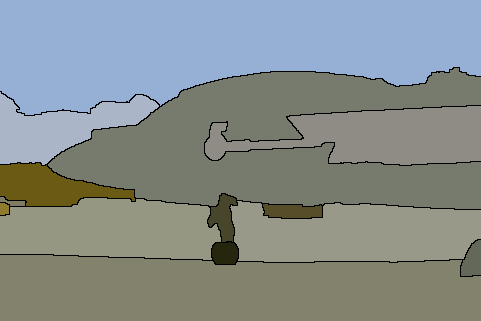
\includegraphics[width=2cm]{scale-aware/fig/visual_result/visual_result_1_7.png} \hspace{-4mm}
\\
\hspace{-2mm}
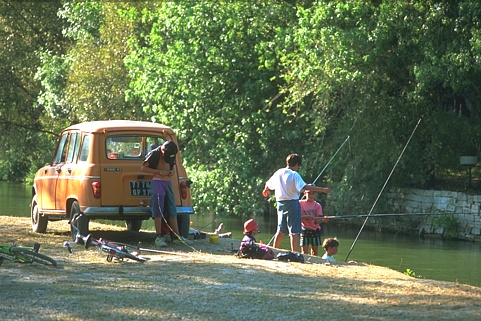
\includegraphics[width=2cm]{scale-aware/fig/visual_result/visual_result_2_1.png} \hspace{-4mm}
&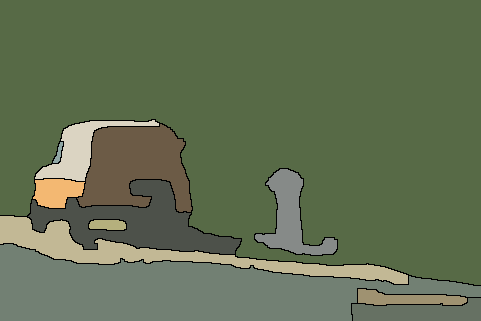
\includegraphics[width=2cm]{scale-aware/fig/visual_result/visual_result_2_2.png} \hspace{-4mm}
&
\includegraphics[width=2cm]{scale-aware/fig/visual_result/visual_result_2_3.png} \hspace{-4mm}
&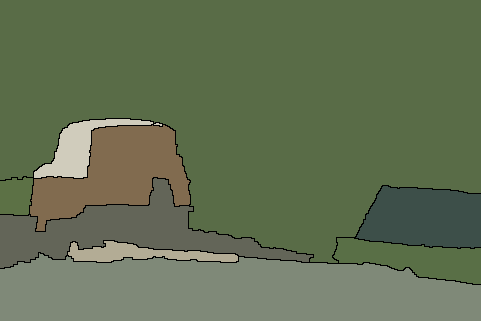
\includegraphics[width=2cm]{scale-aware/fig/visual_result/visual_result_2_4.png}\hspace{-4mm}
&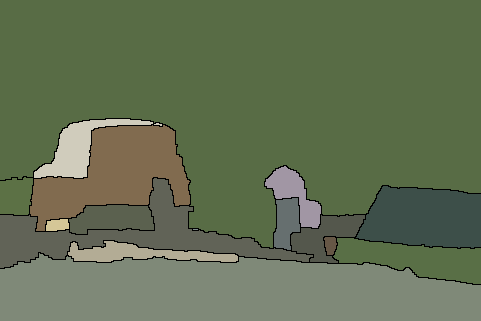
\includegraphics[width=2cm]{scale-aware/fig/visual_result/visual_result_2_5.png} \hspace{-4mm}
&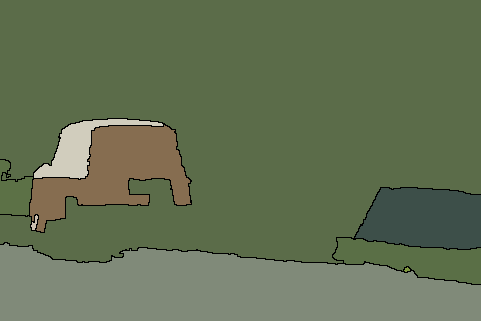
\includegraphics[width=2cm]{scale-aware/fig/visual_result/visual_result_2_6.png} \hspace{-4mm}
&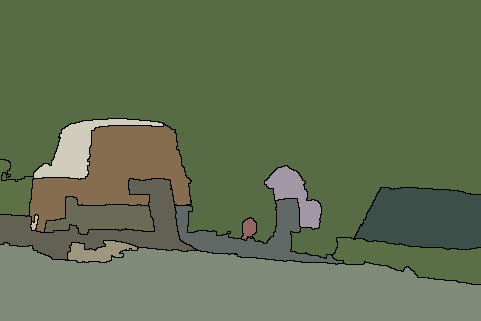
\includegraphics[width=2cm]{scale-aware/fig/visual_result/visual_result_2_7.png} \hspace{-4mm}
\\
\hspace{-2mm}
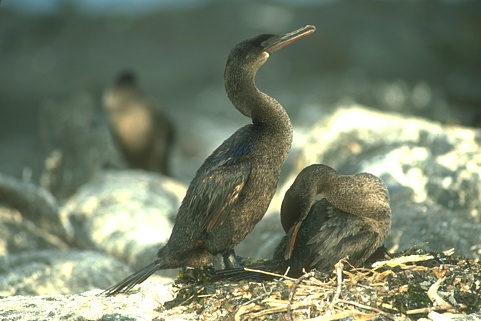
\includegraphics[width=2cm]{scale-aware/fig/visual_result/visual_result_3_1.png} \hspace{-4mm}
&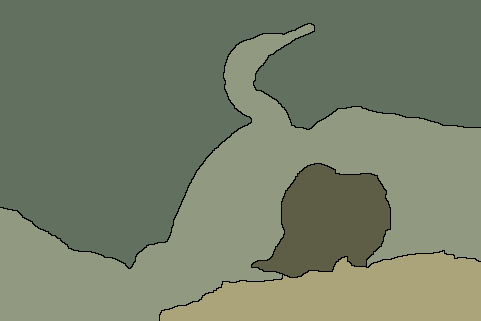
\includegraphics[width=2cm]{scale-aware/fig/visual_result/visual_result_3_2.png} \hspace{-4mm}
&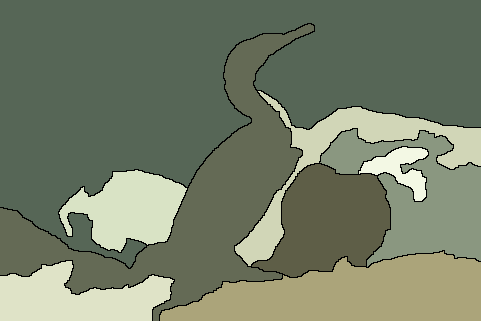
\includegraphics[width=2cm]{scale-aware/fig/visual_result/visual_result_3_3.png} \hspace{-4mm}
&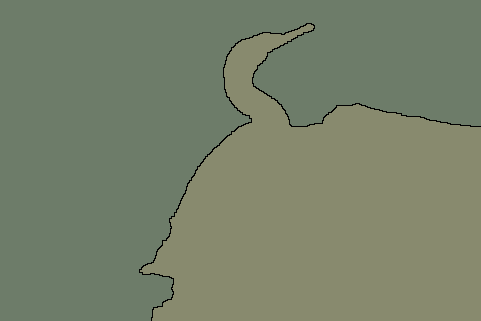
\includegraphics[width=2cm]{scale-aware/fig/visual_result/visual_result_3_4.png}\hspace{-4mm}
&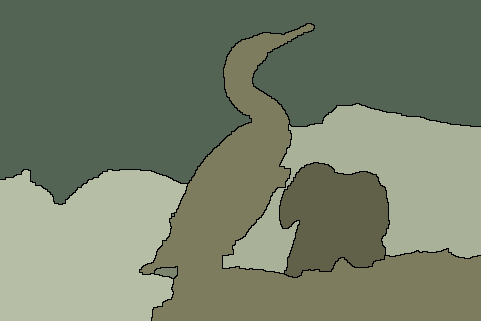
\includegraphics[width=2cm]{scale-aware/fig/visual_result/visual_result_3_5.png}\hspace{-4mm}
&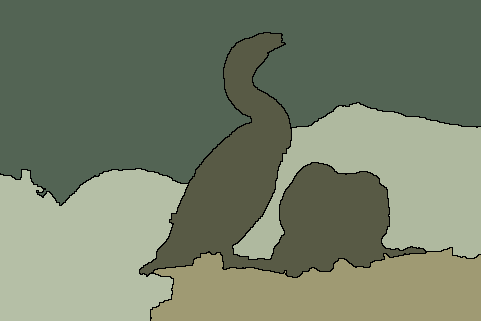
\includegraphics[width=2cm]{scale-aware/fig/visual_result/visual_result_3_6.png}\hspace{-4mm}
&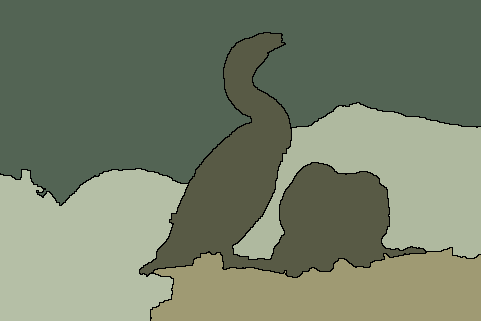
\includegraphics[width=2cm]{scale-aware/fig/visual_result/visual_result_3_7.png}\hspace{-4mm}
\\
\hspace{-2mm}
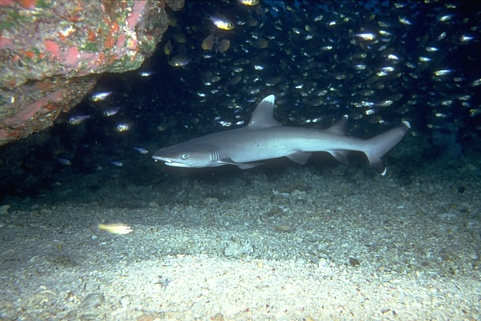
\includegraphics[width=2cm]{scale-aware/fig/visual_result/visual_result_4_1.png} \hspace{-4mm}
&
\includegraphics[width=2cm]{scale-aware/fig/visual_result/visual_result_4_2.png}\hspace{-4mm}
&
\includegraphics[width=2cm]{scale-aware/fig/visual_result/visual_result_4_3.png} \hspace{-4mm}
&
\includegraphics[width=2cm]{scale-aware/fig/visual_result/visual_result_4_4.png}\hspace{-4mm}
&
\includegraphics[width=2cm]{scale-aware/fig/visual_result/visual_result_4_5.png}\hspace{-4mm}
&
\includegraphics[width=2cm]{scale-aware/fig/visual_result/visual_result_4_6.png}\hspace{-4mm}
&
\includegraphics[width=2cm]{scale-aware/fig/visual_result/visual_result_4_7.png}\hspace{-4mm}
\\
\hspace{-2mm}
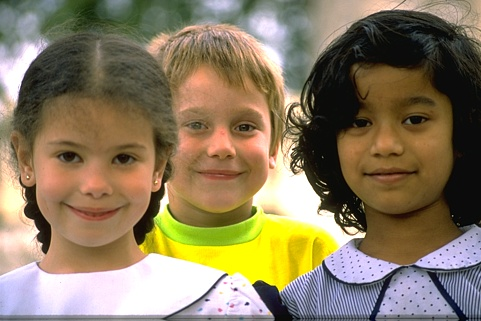
\includegraphics[width=2cm]{scale-aware/fig/visual_result/visual_result_5_1.png}\hspace{-4mm}
&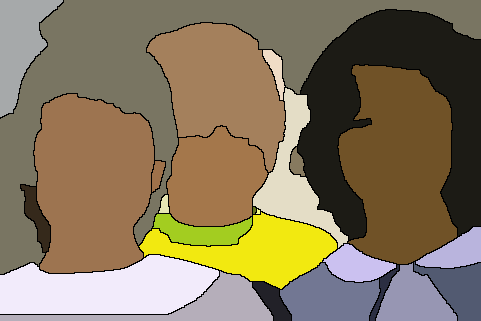
\includegraphics[width=2cm]{scale-aware/fig/visual_result/visual_result_5_2.png}\hspace{-4mm}
&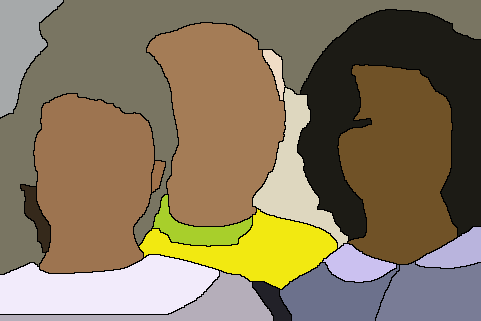
\includegraphics[width=2cm]{scale-aware/fig/visual_result/visual_result_5_3.png}\hspace{-4mm}
&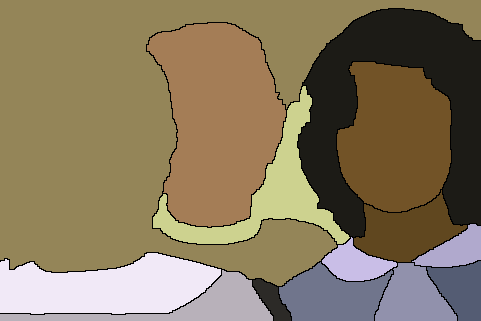
\includegraphics[width=2cm]{scale-aware/fig/visual_result/visual_result_5_4.png} \hspace{-4mm}
&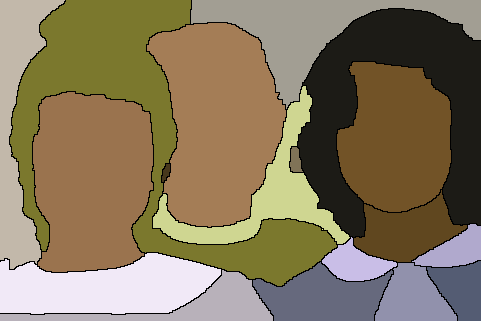
\includegraphics[width=2cm]{scale-aware/fig/visual_result/visual_result_5_5.png}\hspace{-4mm}
&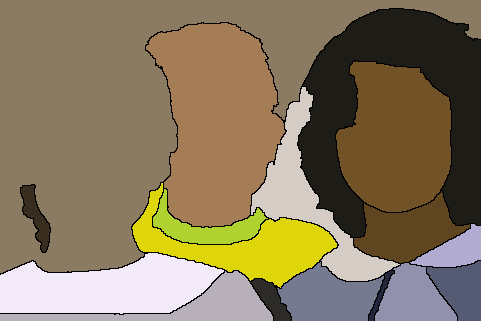
\includegraphics[width=2cm]{scale-aware/fig/visual_result/visual_result_5_6.png}\hspace{-4mm}
&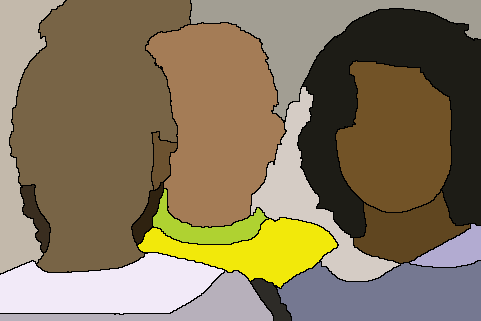
\includegraphics[width=2cm]{scale-aware/fig/visual_result/visual_result_5_7.png}\hspace{-4mm}
\\
\hspace{-2mm}
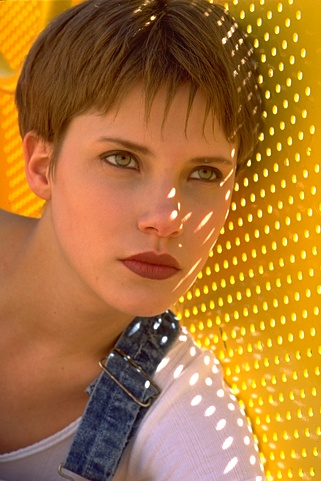
\includegraphics[width=2cm]{scale-aware/fig/visual_result/visual_result_6_1.png}\hspace{-4mm}
&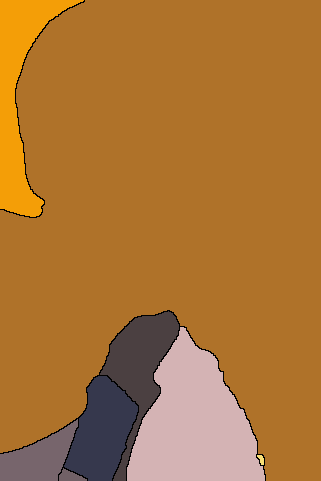
\includegraphics[width=2cm]{scale-aware/fig/visual_result/visual_result_6_2.png}\hspace{-4mm}
&\includegraphics[width=2cm]{scale-aware/fig/visual_result/visual_result_6_3.png}\hspace{-4mm}
&\includegraphics[width=2cm]{scale-aware/fig/visual_result/visual_result_6_4.png}\hspace{-4mm}
&\includegraphics[width=2cm]{scale-aware/fig/visual_result/visual_result_6_5.png}\hspace{-4mm}
&\includegraphics[width=2cm]{scale-aware/fig/visual_result/visual_result_6_6.png}\hspace{-4mm}
&\includegraphics[width=2cm]{scale-aware/fig/visual_result/visual_result_6_7.png}\hspace{-4mm}
\\
\end{tabular}
\end{center}
\caption{Comparison of segmentation results, hierarchies are flattened by optimal dataset scale(ODS).}
\label{fig:visualresult}
\end{figure*}


\subsection{Evaluation towards Object Segmentation}
Segmentation \textit{per se} is rarely the final objective of real
applications, it is rather a middle tool towards, for instance, object
segmentation~\cite{arbelaez2014multiscale} or semantic
segmentation~\cite{Lempitsky2011}.  This section is devoted to show
that better aligned hierarchies also help in this scenario.

In this case we firstly perform the evaluation using the object annotations
provided on the BSDS300 set by~\cite{Endres2014} (we retrain on only BSDS300 train instead of BSDS500).
The intuitive idea is to measure how well we can segment these objects by
\textit{selecting} regions from the different flattened hierarchies.

Figure~\ref{fig:qual_vs_regs} shows the achievable quality
that an oracle could reached if selecting the regions from the
original hierarchies or the ones with our newly-proposed alignment.
The X axis corresponds to the number of needed regions, \ie, the lower
the better.

We can observe that the aligned hierarchies consistently need less
regions to get the same quality in all the tested hierarchies.  In
PMI, for instance, we need to select 5 regions to achieve the same
quality that we can get with 4 on the aligned hierarchy. The
combinatorial space of all possible 4-region combinations is
significantly smaller and thus the search is more probable to
succeed. On the other direction, if we limit the number of regions we
get improvements up to 3 points (9\%) in the achievable quality.

To further illustrates the scalability of the hierarchy alignment on larger dataset, we evaluated our alignment algorithm on Pascal VOC 2012 Segmentation set~\cite{everingham2010pascal} and Microsoft COCO~\cite{lin2014microsoft}. We retrain our scale predictor using the training set of Pascal 2012. In Pascal 2012 dataset, only the segmentation of foreground objects are given, in contrast to BSDS which is fully annotated. Thus during training we only consider all the segments that have overlap with foreground object annotations. The scale predictor is trained as described in Sec~\ref{sec:scale}, the only difference is that $\mathbf{g}$ can only be foreground object. This strategy introduces extra bias towards foreground objects, because no information about the scale of background is given in the training process. However, we are still able to improve alignment of segmentation hierarchies . As shown in Fig.~\ref{fig:qual_vs_regs}, we see that for the range of 2-3 regions (the one in which the MCG object proposal work), the aligned hierarchy provides a 2.5-point improvement ($\sim$6\%), which shows that our method generalizes to larger datasets. 

\subsection{Running Time}
Our approach takes approximately 3 seconds in total for each image, of which $2.39$
seconds are spent on feature extraction from the segments. The prediction
of regression forest takes about $0.45$ seconds, and the dynamic
programming takes $0.05$ seconds for the inference. Finally, $0.11$
seconds are spent for re-scaling the UCM.
All times are measured on a standard desktop machine.

\begin{figure*}[tb]
\begin{center}
\begin{tabular}{c}
\includegraphics[width=14.7cm]{scale-aware/fig/vis/stack_1.png} \\
\includegraphics[width=14.7cm]{scale-aware/fig/vis/stack_2.png}
\end{tabular}
\end{center}
\caption{Results of MCG(first row) and MCG results improved by our approach(second row). Original images are shown in the left most. Segmentations of optimal-dataset-sclae(ODS) are given in the middle. And from left to right are different scales, from fine to coarse. Red bounding box indicates the scale with best results achieved by MCG, and blue box for ours. It can be seen that our approach provides better alignment, both across images and within one image. }
\label{fig:mcg_vis2}
\end{figure*}



% \begin{figure*}
% \begin{center}
% \begin{tabular}{c}
% \includegraphics[width=17cm]{scale-aware/fig/vis/70090.png} \\
% \includegraphics[width=17cm]{scale-aware/fig/vis/388006.png} \\
% \includegraphics[width=17cm]{scale-aware/fig/vis/48017.png} \\
% \includegraphics[width=17cm]{scale-aware/fig/vis/196062.png}
% \end{tabular}
% \end{center}
% \caption{Results of MCG(first row) and MCG results improved by our approach(second row). Original images are shown in the left most. Segmentations of optimal-dataset-sclae(ODS) are given in the middle. And from left to right are different scales, from fine to coarse. Red bounding box indicates the scale with best results. It can be seen that our approach provides better alignment, both across images and within one image. }
% \label{fig:mcg_vis1}
% \end{figure*}


\section{Conclusion}
\label{sec:conclusions}
In this work, we presented a novel technique to align segmentation
hierarchies. We proposed a method to learn and predict the scale of
segments. We formulated the scale prediction for the segments in
a hierarchy as a graph label problem, which is solved by dynamic
programming. With the labeled scales as constraints, we then re-align
the segmentation hierarchies by stretching the UCM maps. The method
is evaluated on four different segmentation hierarchies on BSDS500, and it
consistently improves their quality.  We also showed
that the improvement of segmentation hierarchies by our alignment is
reflected well to a higher-level task of getting object segmentations.

%{\small
%\bibliographystyle{ieee}
%\bibliography{egbib}
%}
%
%\end{document}
